\setchapterstyle{kao}
\setchapterpreamble[u]{\margintoc}

\chapter{Heavy Neutral Lepton Signal Simulation}
\labch{signal_simulation}

After the SM simulation generation and the default low energy event selection and processing chain were introduced in the previous \refch{simulation_and_processing}, the focus will now be on the central part of this thesis - the HNL signal simulation. Since this is the first attempt of performing a search for HNLs with IceCube DeepCore, there was no prior knowledge of the expected performance nor the event expectation and the simulation had to be developed from scratch. Two avenues of simulation generation were pursued in parallel; a collection of model independent simulation sets was realized and is explained in \refsec{model_independent_simulation} and the physically accurate model dependent simulation is described in \refsec{model_specific_simulation}.


\section{Model Independent Simulation} \labsec{model_independent_simulation}

To investigate the potential of IceCube to detect HNLs by identifying the unique double cascade morphology explained in \refsec{double_cascade_morphology}, it is very valuable to have simulation sets where the double cascade kinematics can be controlled directly. In a realistic model the decay kinematics and the absolute event expectation all depend on the specific model parameters chosen (see \refsec{hnl_theory}). To decouple the simulation from a specific model, a model independent double cascade generator was developed and will be explained in the following sections. Using these sets, the performance of IceCube DeepCore to detect low energetic double cascades, dependent on their properties, is studied in \refch{double_cascade_performance}. 


\subsection{Generator Functions}

\todo{Throw the generator functions into a public repo (with author+copyright) and link it here}

In order to produce the model independent simulation sets a series of generator functions was implemented in \textsc{Python} \sidecite{python}.
% The collection of functions can be found in \href{}{this public repository.}
A few independent functions are needed to perform the sampling based on a random variable between \SIrange[range-phrase={~and~}]{0}{1}{} as input. There is a simple function to return a random sign ($+1/-1$) and two functions to sample from a power law and an exponential distribution. The inputs are the wanted sampling range and the power law index or the exponential decay constant, respectively. They both apply the inverse transformation method.

Additionally, there are some functions that are IceCube specific. Two functions are implemented to transform a direction in zenith/azimuth angles a direction vector and vice versa. There is a function to create an EM cascade particle from a position, direction, energy, and time and another to produce an arbitrary list of EM cascades, given the list of input parameters, and adding it to the current IceCube event. Based on these, any specific simulation set can be produced by defining the sampling distributions and number of cascades to be placed in each event and then calling the generator functions.

% \marginnote{
  \begin{kaobox}[frametitle=IceCube software framework]
    Add a box with some information on the \href{https://github.com/icecube/icetray-public}{(public) icetray} software and how the above is using \href{https://docs.icecube.aq/icetray/main/projects/dataclasses/particle.html#i3particle}{I3Particle}, \href{https://docs.icecube.aq/icetray/main/projects/dataclasses/i3mctree.html#i3mctree}{I3MCTree}, and \href{https://docs.icecube.aq/icetray/main/projects/icetray/classes/i3frame.html#index-0}{I3Frame} objects.
  \end{kaobox}
% }


\subsection{Simplistic Sets}

To test the implemented generator functions and investigate some idealistic double cascade event scenarios, two sets are produced for straight up-going events that are centered on a string and horizontal events located inside DeepCore.

\todo{Make my own DC string positions/distances plot}
\begin{figure}[h]
    \centering
    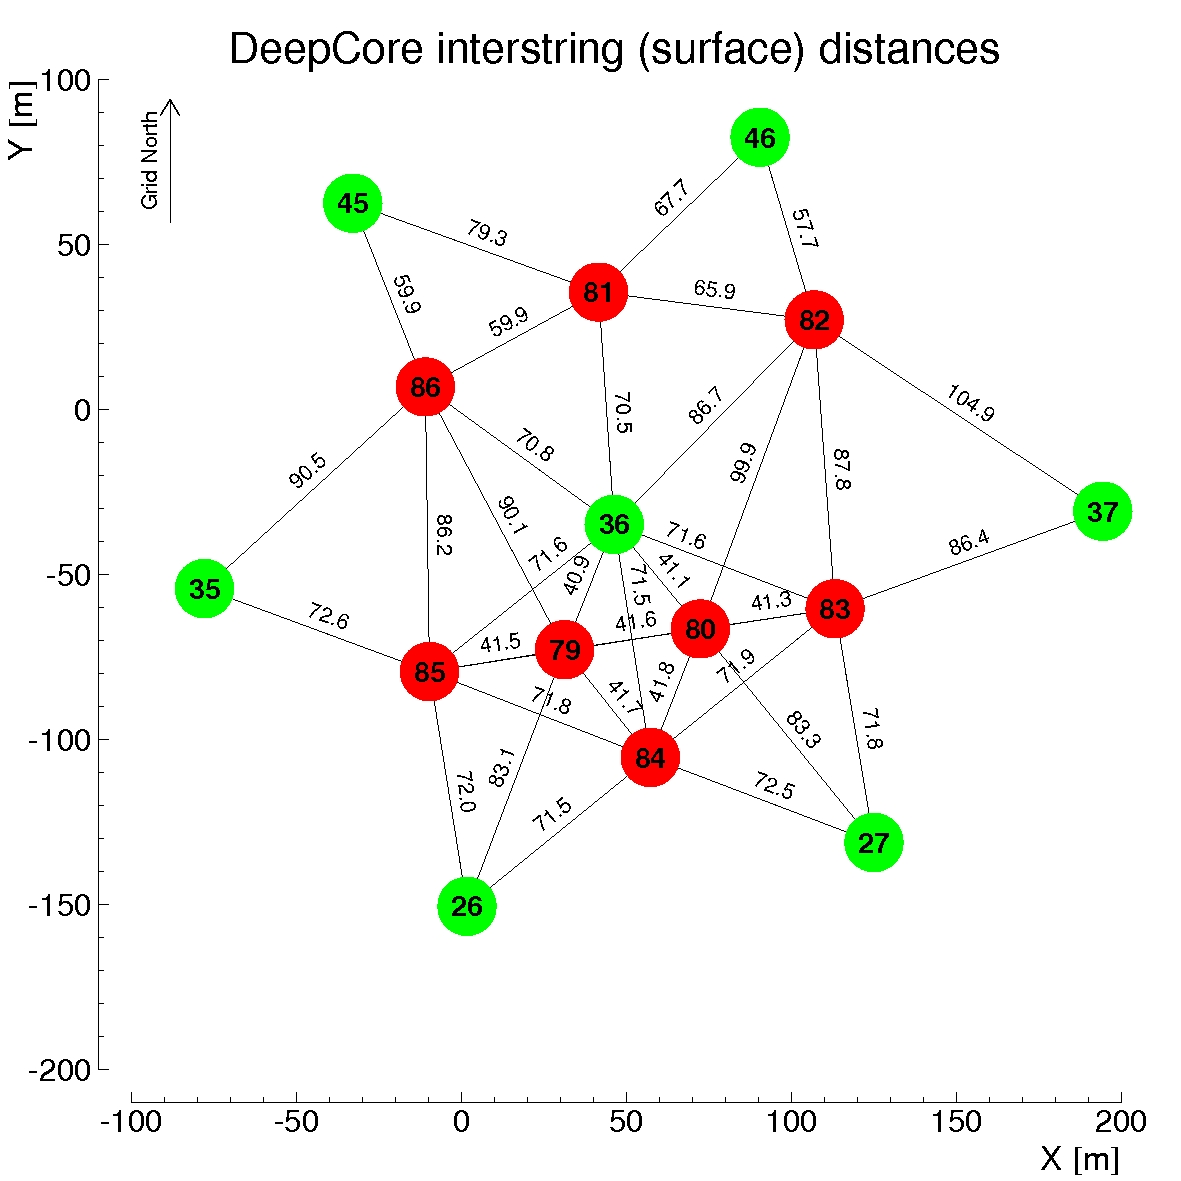
\includegraphics{figures/icecube_deepcore/deepcore_surface_distances.jpg}
    \caption[xx]{Horizontal positions and distances between DeepCore strings. Red strings are instrumented more densely (vertically) and partially with higher quantum efficiency (HQE) DOMs.}
    \labfig{deepcore_distances}
\end{figure}

The first set is used to investigate one of the best possible cases to detect a double cascade, where both cascades are placed on a DeepCore string (namely string 81) and the directions are directly up-going. The horizontal positions and distances of all DeepCore fiducial volume strings are shown in \reffig{deepcore_distances}. As already mentioned in \refsec{deepcore}, DeepCore strings have higher quantum efficiency DOMs and a denser vertical spacing. The $(x,y)$ position is fixed to the center of string 8 while the $z$ position of each cascade is sampled uniformly along the strings $z$ elongation and the energies are sampled uniformly between \SIrange{0.0}{60.0}{\gev}. The specific sampling distributions/values for the cascades are listed in \reftab{hnl_simplified_set_sampling_distributions}. The order of the cascades is chosen such that the lower one is first ($t_0=0.0$) and the upper one is second ($t_1=L/c$), assuming the speed of light $c$ as speed of the heavy mass state, traveling between the two cascades.
% The generation level distributions of the up-going set are shown in \reffig{upgoing_string81_gen_distris}.

\begin{table}
    \small
        \begin{tabular}{ llll }
        \hline\hline
        \textbf{Set} & \textbf{Variable} & \textbf{Distribution} & \textbf{Range/Value} \\
        \hline\hline
        \multicolumn{2}{l}{Up-going} && \\
        \hline
        & energy & uniform & \SIrange{0.0}{60.0}{\gev} \\
        & zenith & fixed & \SI{180.0}{\degree} \\
        & azimuth & fixed & \SI{0.0}{\degree} \\
        & $x,y$ position & fixed & (41.6, 35.49)\,\si{\metre} \\
        & $z$ position & uniform & \SIrange{-480.0}{-180.0}{\metre} \\
        \hline
        \multicolumn{2}{l}{Horizontal} && \\ 
        \hline
        & energy & uniform & \SIrange{0.0}{60.0}{\gev} \\
        & zenith & fixed & \SI{90.0}{\degree} \\
        & azimuth & uniform & \SIrange{0.0}{360.0}{\degree} \\
        & $x,y$ position & uniform (circle) & $c$=(46.29, -34.88)\,\si{\metre}, $r$=\SI{150.0}{\metre} \\
        & $z$ position & fixed & \SI{-330.0}{\metre} \\
        \hline
        \end{tabular}
    \caption[xx]{Sampling distributions of up-going, string 81 centered and horizontal simulation generation.}
    \labtab{hnl_simplified_set_sampling_distributions}
\end{table}

\todo{fix caption for simplistic sampling distris}

The second set is used to investigate the effect of the tilt of the double cascade and the reconstruction performance for horizontal events. The cascades are placed uniformly on a circle with centered in DeepCore. The direction is always horizontal and azimuth is defined by the connecting vector of both cascade positions. The energies are again sampled uniformly between \SIrange{0.0}{60.0}{\gev} and the detailed sampling distributions/values are also listed in \reftab{hnl_simplified_set_sampling_distributions}.
% The generation level distributions of the horizontal set are shown in \reffig{horizontal_gen_distris}.


\subsection{Realistic Set}

To thoroughly investigate the potential of IceCube DeepCore to detect double cascade events, a more realistic simulation set is produced that aims to be as close as possible to the expected signal simulation explained in \refsec{model_specific_simulation}, while still allowing some freedom to control the double cascade kinematics. For this purpose the total energy is sampled from an $E^{-2}$ power law, mimicking the energy spectrum of the primary neutrinos as stated in \refsec{neutrino_generation}. Although in the realistic process described in \refsec{model_specific_simulation} the energy is distributed in a more complex way into the two cascades and secondary particles, it is a good approximation to simply divide the total energy into two parts. This is done by randomly assigning a fraction between \SIrange[range-phrase={~and~}]{0}{100}{\percent} to one cascade and the remaining part to the other cascade. In this way the whole sample covers various cases of energy distributions between the two cascades. To efficiently generate events in a way that produces distributions similar to what would be observed with DeepCore, one of the cascades positions is sampled inside the DeepCore volume by choosing is coordinates randomly on a cylinder that is centered in DeepCore. This partly imitates a trigger condition of one cascade always being inside the DeepCore fiducial volume. By choosing the direction of the event sampling zenith and azimuth uniformly between \SIrange[range-phrase={~and~}]{70}{180}{\degree} and \SIrange[range-phrase={~and~}]{0}{360}{\degree}, respectively, the position of the other cascade can be inferred for a given decay length. The length is sampled from an exponential distribution, which would be expected for the decaying heavy mass state. Based on the direction and the decay length, the position of the other cascade is found, assuming a travel speed of $c$ and randomly chosing whether the cascade position that was sampled is the first cascade or the second and then assigning the other cascade position accordingly. The sampling distributions/values are listed in \reftab{hnl_realistic_set_sampling_distributions}.

\begin{table}
    \small
        \begin{tabular}{ llll }
        \hline\hline
        \textbf{Variable} & \textbf{Distribution} & \textbf{Range/Value} \\
        \hline\hline
        energy (total) & power law $E^{-2}$ & \SIrange{1}{1000}{\gev} \\
        decay length & exponential e$^{-0.01L}$ & \SIrange{0}{1000}{\metre} \\
        zenith & uniform & \SIrange{70}{180}{\degree} \\
        azimuth & uniform & \SIrange{0}{360}{\degree} \\
        $x,y$ (one cascade) & uniform (circle) & $c$=(46.29, -34.88)\,\si{\metre}, $r$=\SI{150}{\metre} \\
        $z$ (one cascade) & uniform & \SIrange{-480.0}{-180.0}{\metre}\\
        \hline
        \end{tabular}
    \caption[xx]{xx}
    \labtab{hnl_realistic_set_sampling_distributions}
\end{table}

\todo{fix caption for realistic sampling distris}


\subsection{Generation Level Distributions}

% \begin{figure}[h!]
%     \subfloat[\labfig{upgoing_string81_gen_distris_energies}]{
%         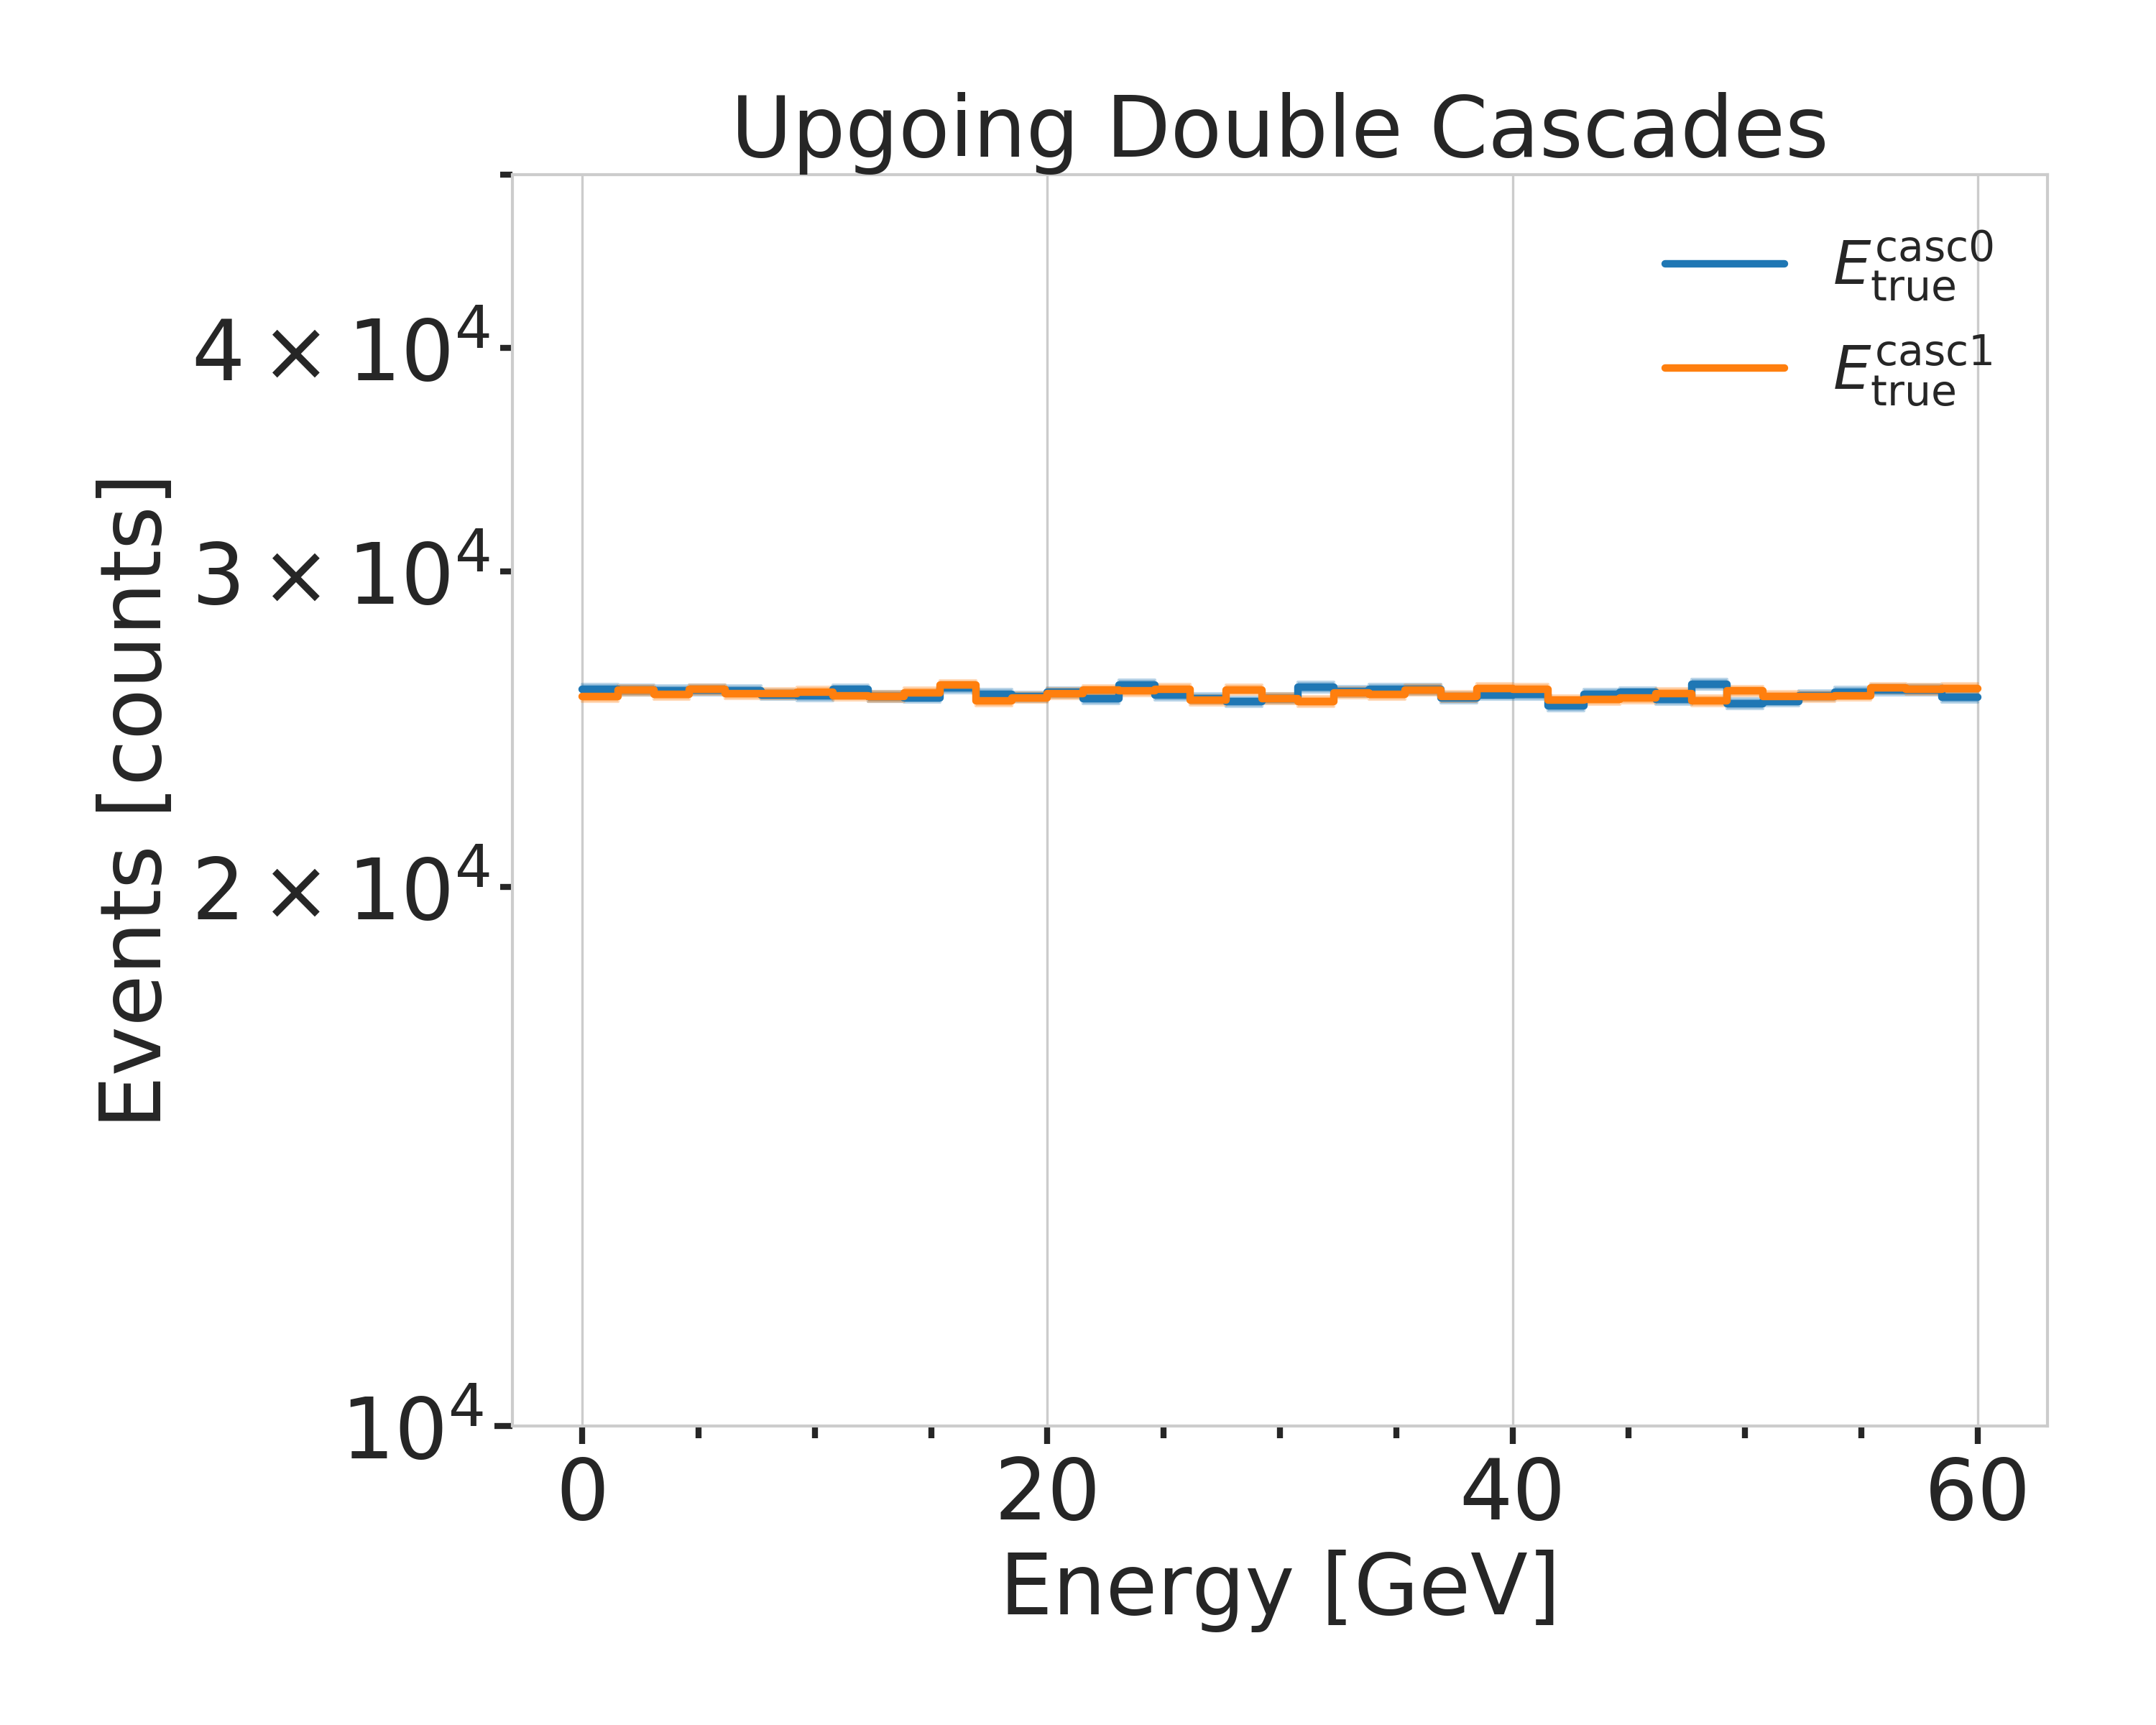
\includegraphics[width=.45\linewidth]{figures/upgoing_string_81_gen_level/1_d_distr_energies_clipped.png}
%     }
%     \subfloat[\labfig{upgoing_string81_gen_distris_depths}]{
%         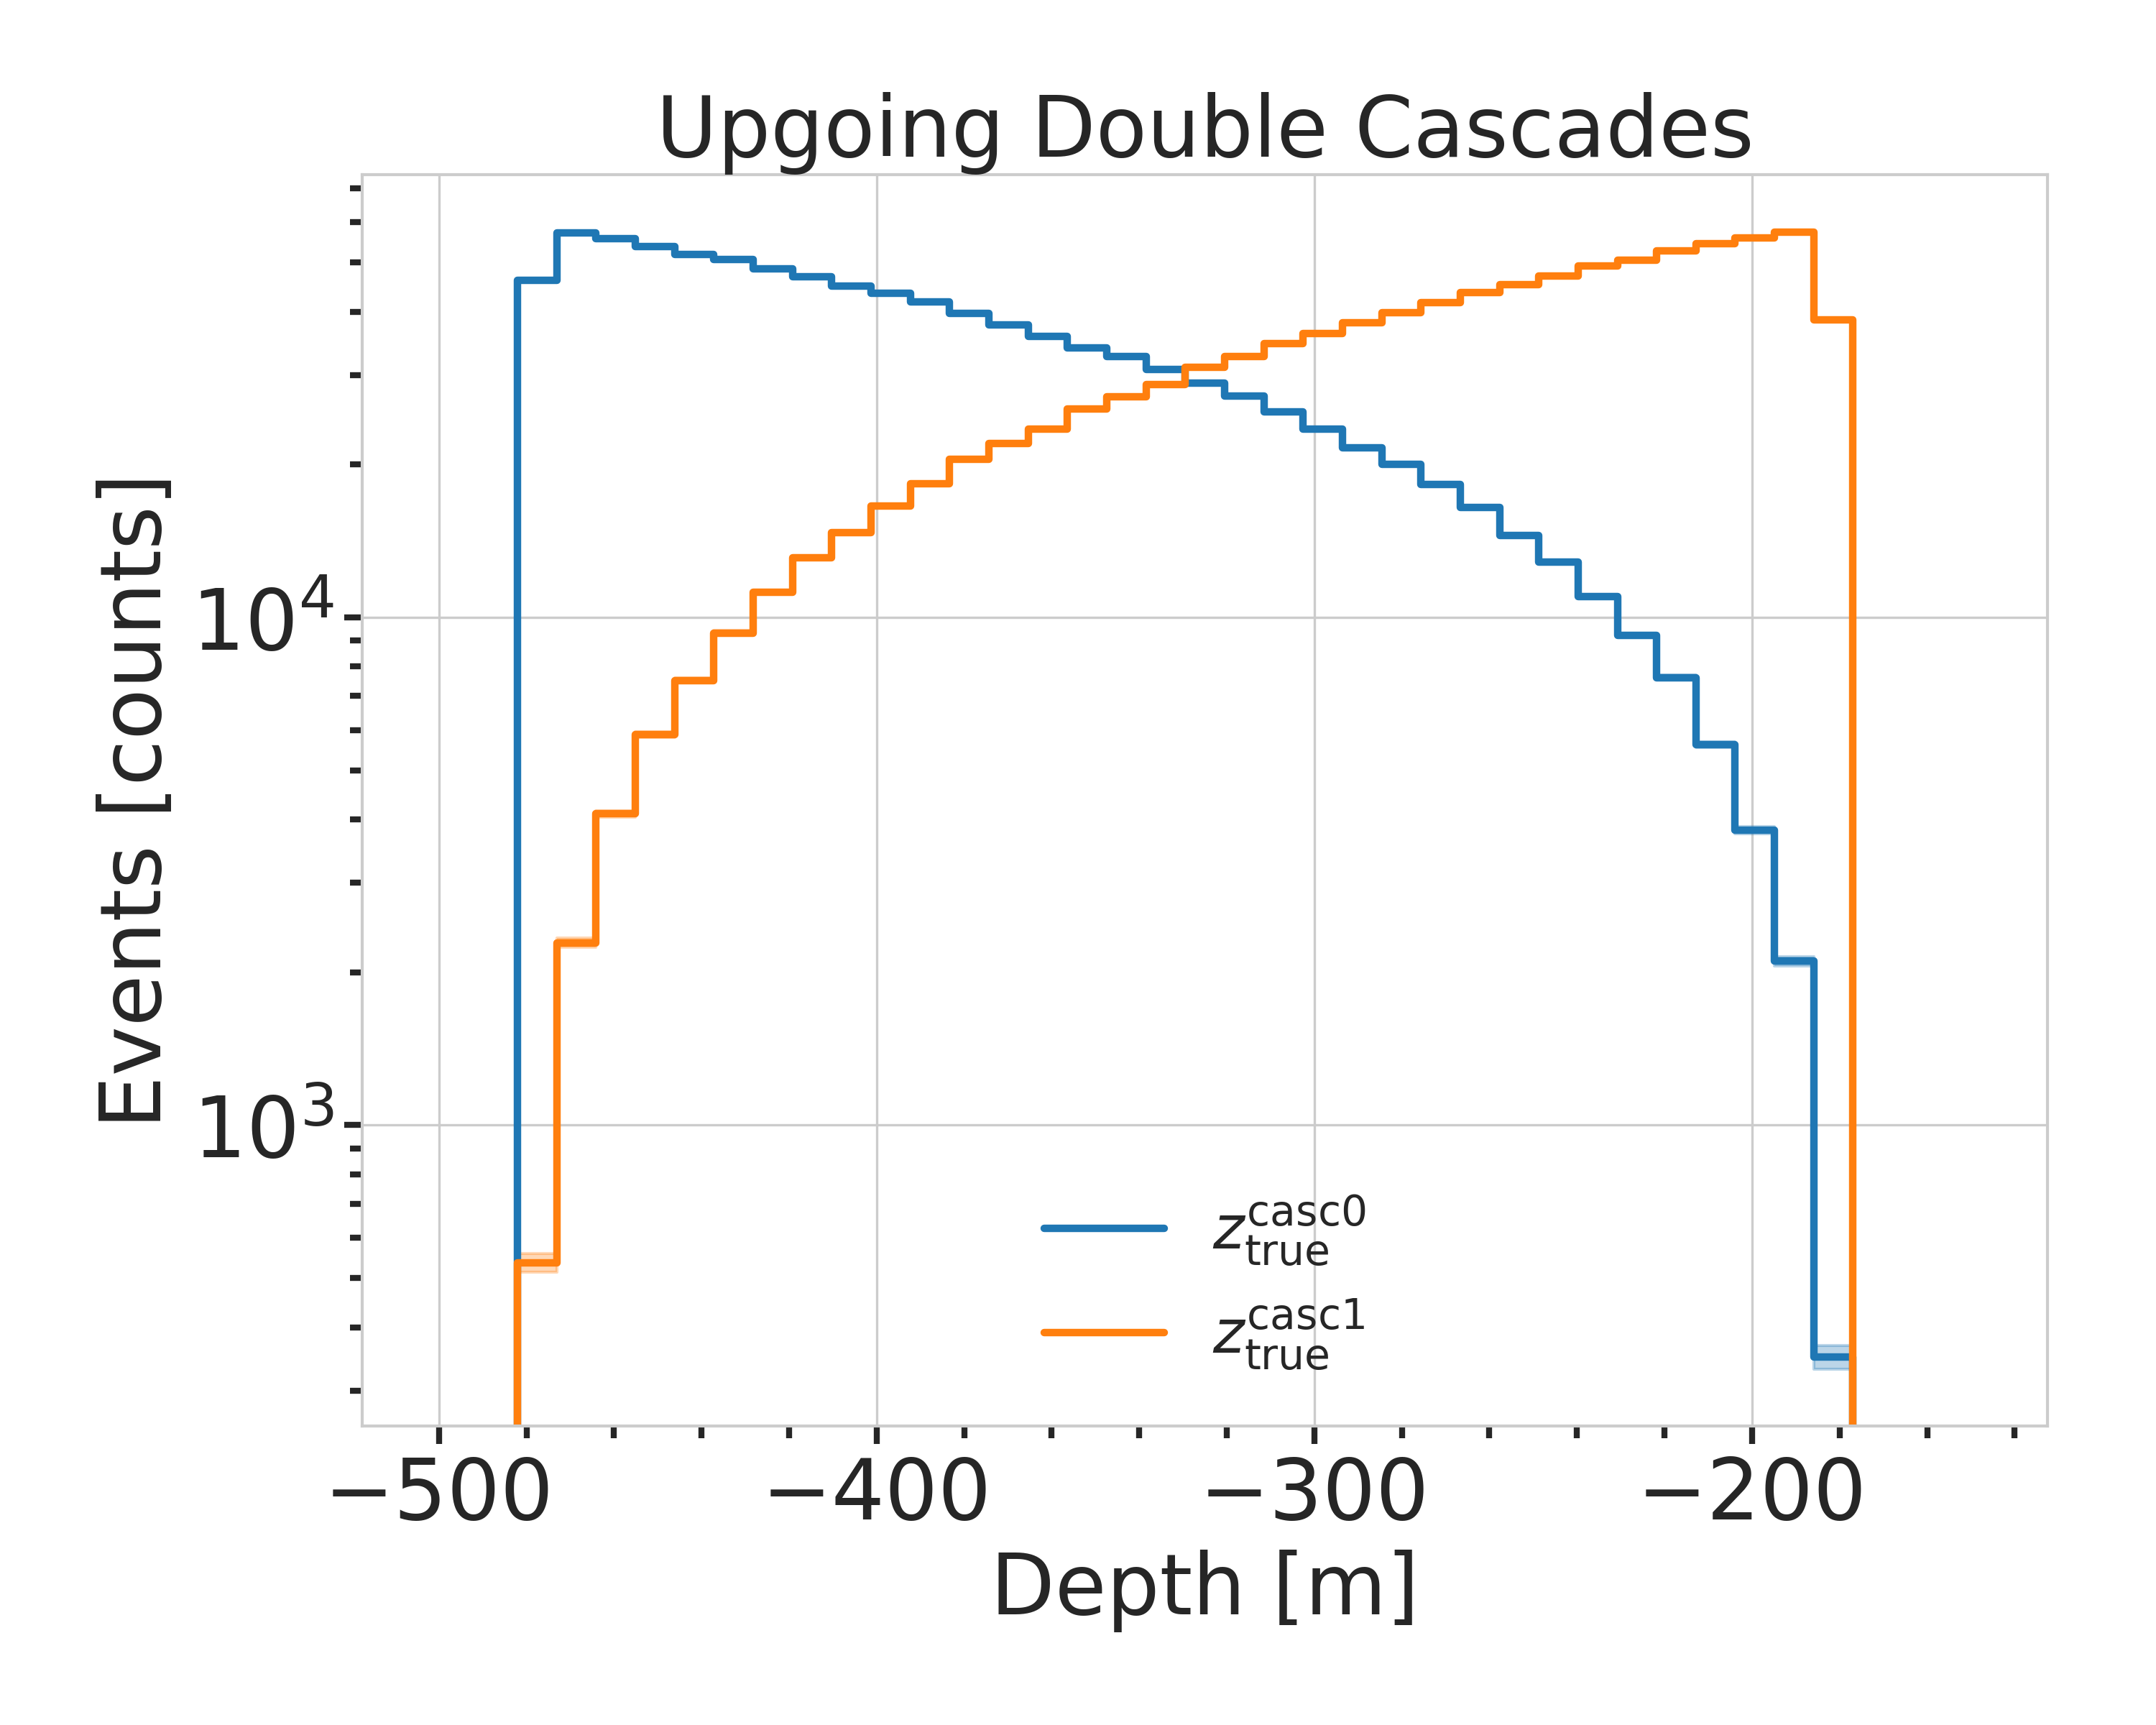
\includegraphics[width=.45\linewidth]{figures/upgoing_string_81_gen_level/1_d_distr_depths_clipped.png}
%     }
%     \\[-2.5ex]
%     \subfloat[\labfig{upgoing_string81_gen_distris_decay_length}]{
%         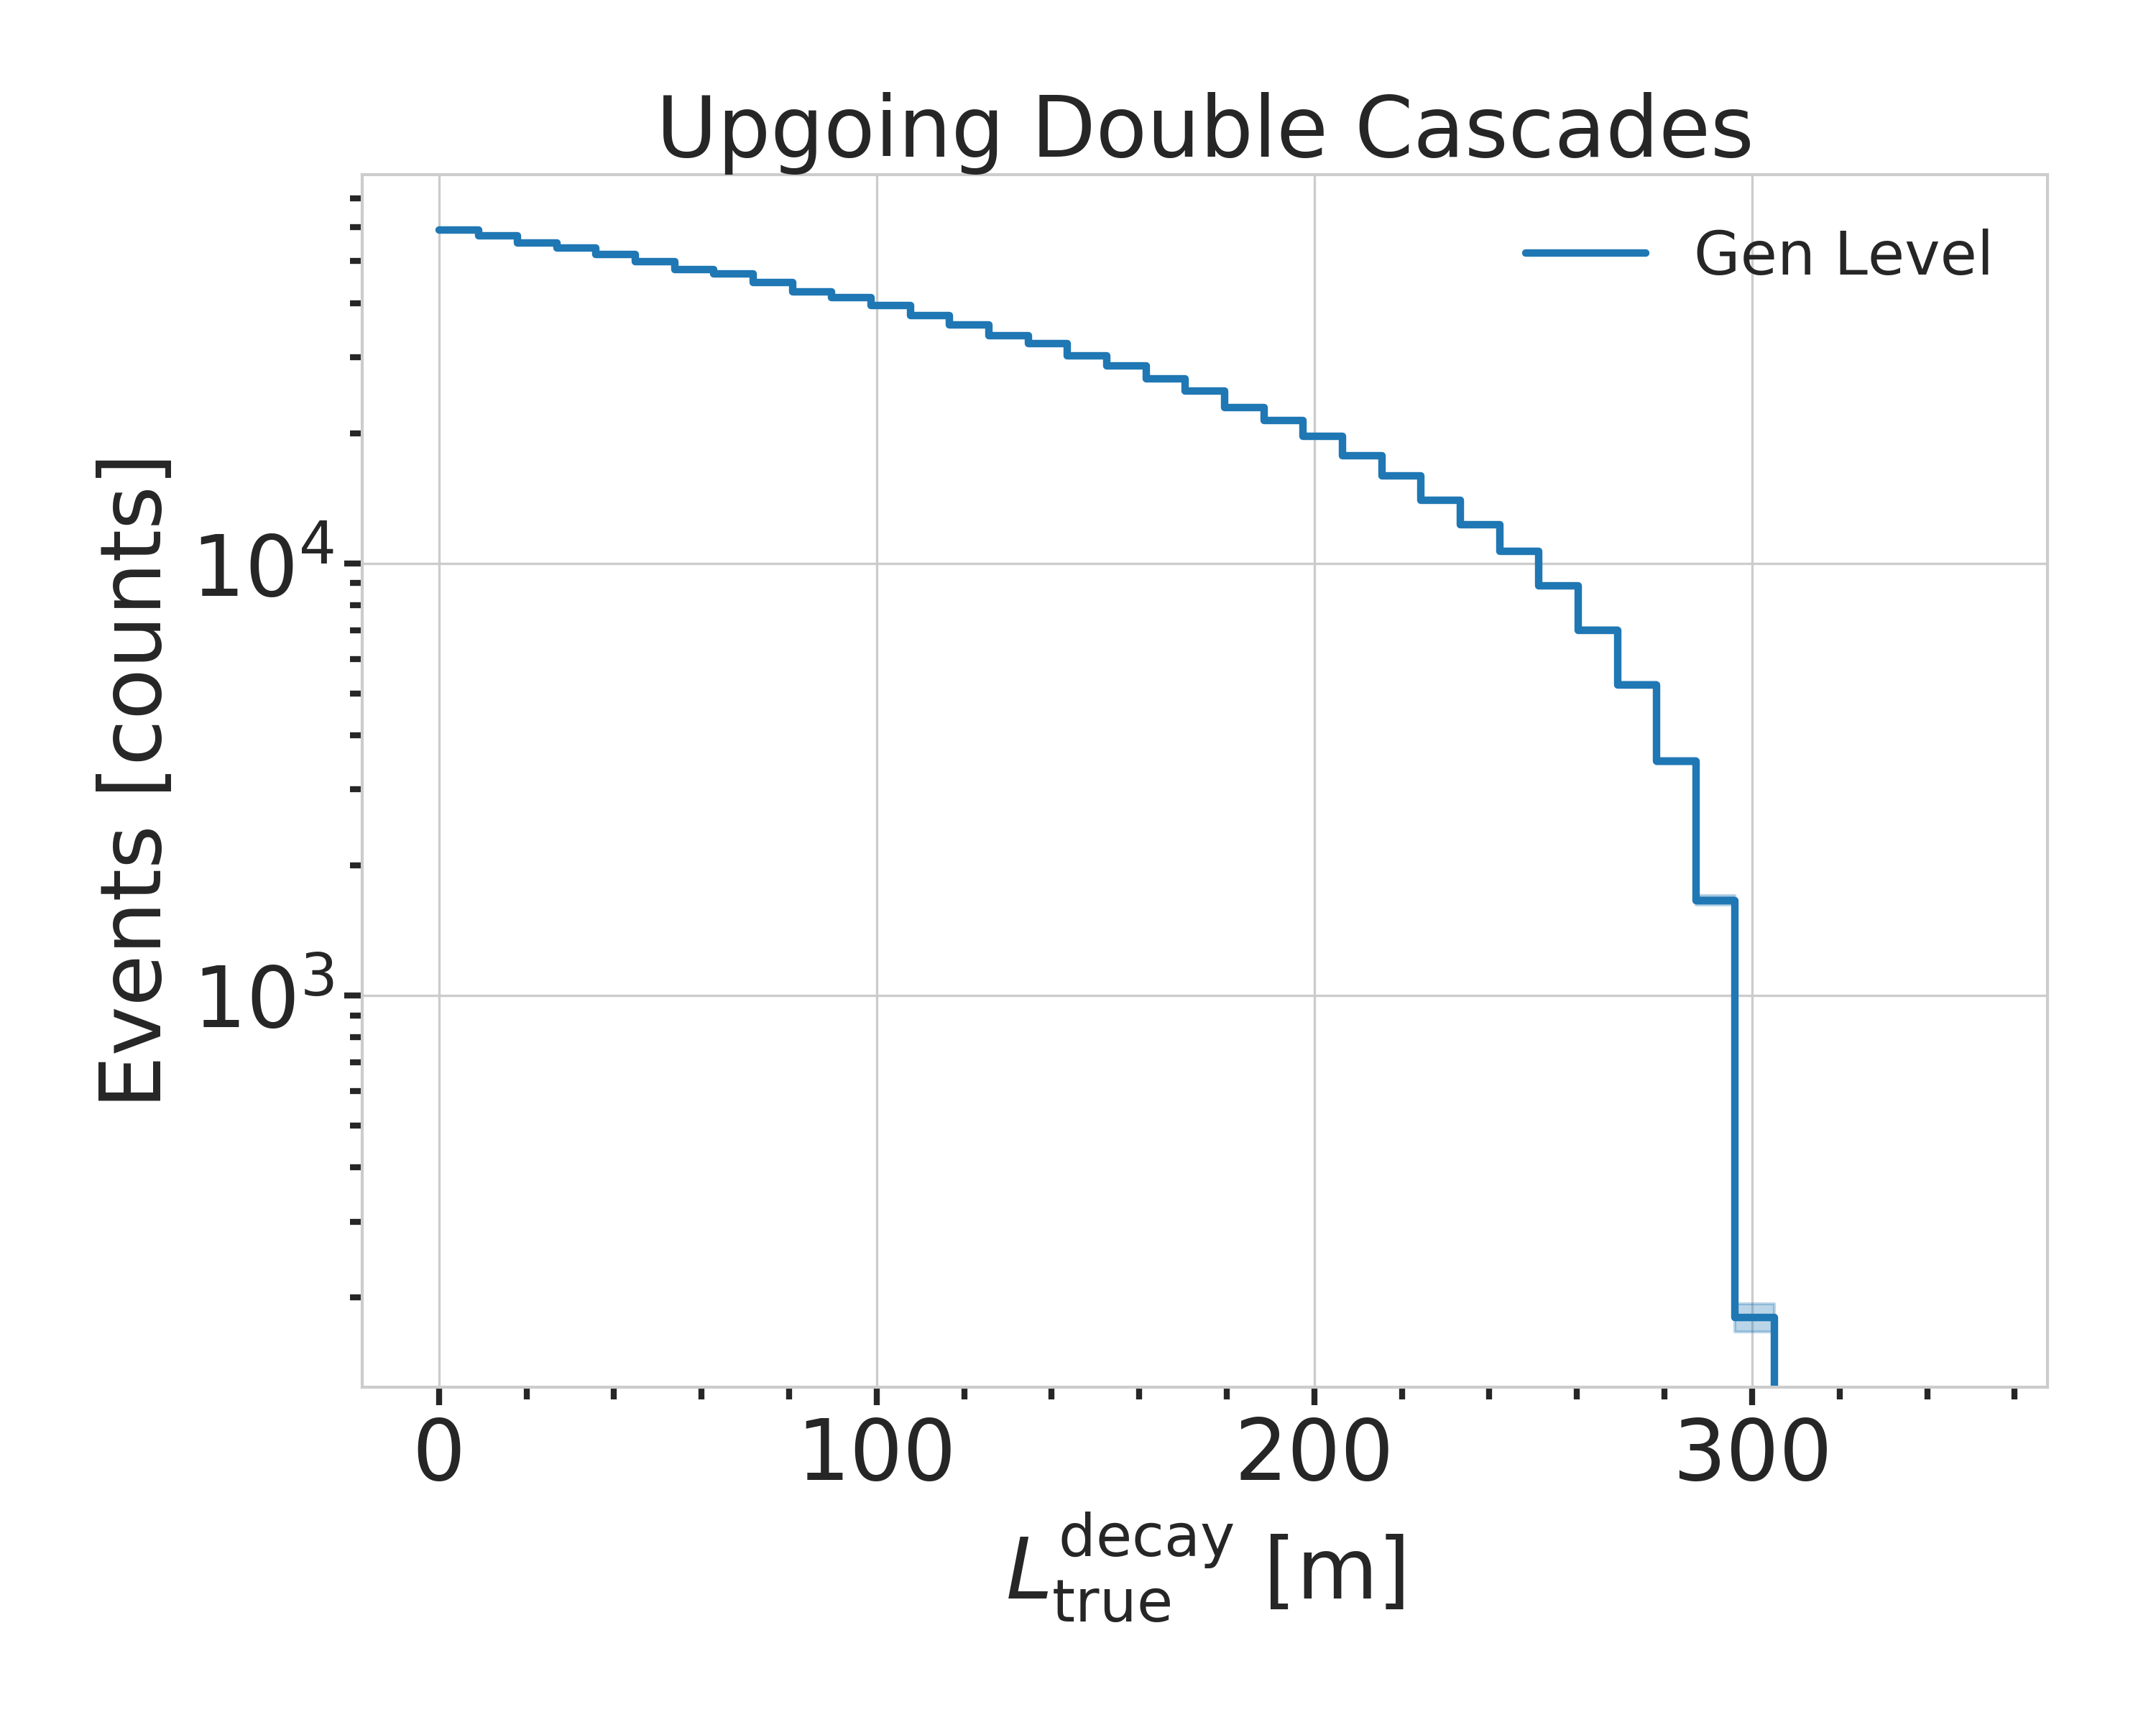
\includegraphics[width=.45\linewidth]{figures/upgoing_string_81_gen_level/1_d_distr_true_decay_length_clipped.png}
%     }
%     \subfloat[\labfig{upgoing_string81_gen_distris_total_energy}]{
%         \includegraphics[width=.45\linewidth]{figures/upgoing_string_81_gen_level/1_d_distr_true_total_energy_clipped.png}
%     }
%     \caption{Generation level distributions of the 1000 files, with 1000 events each of set 194601. Only the parameters that are not fixed to a certain value are shown.}
%     \labfig{upgoing_string81_gen_distris}
% \end{figure}


% \begin{figure}[h!]
%     \subfloat[\labfig{horizontal_gen_distris_energies}]{
%         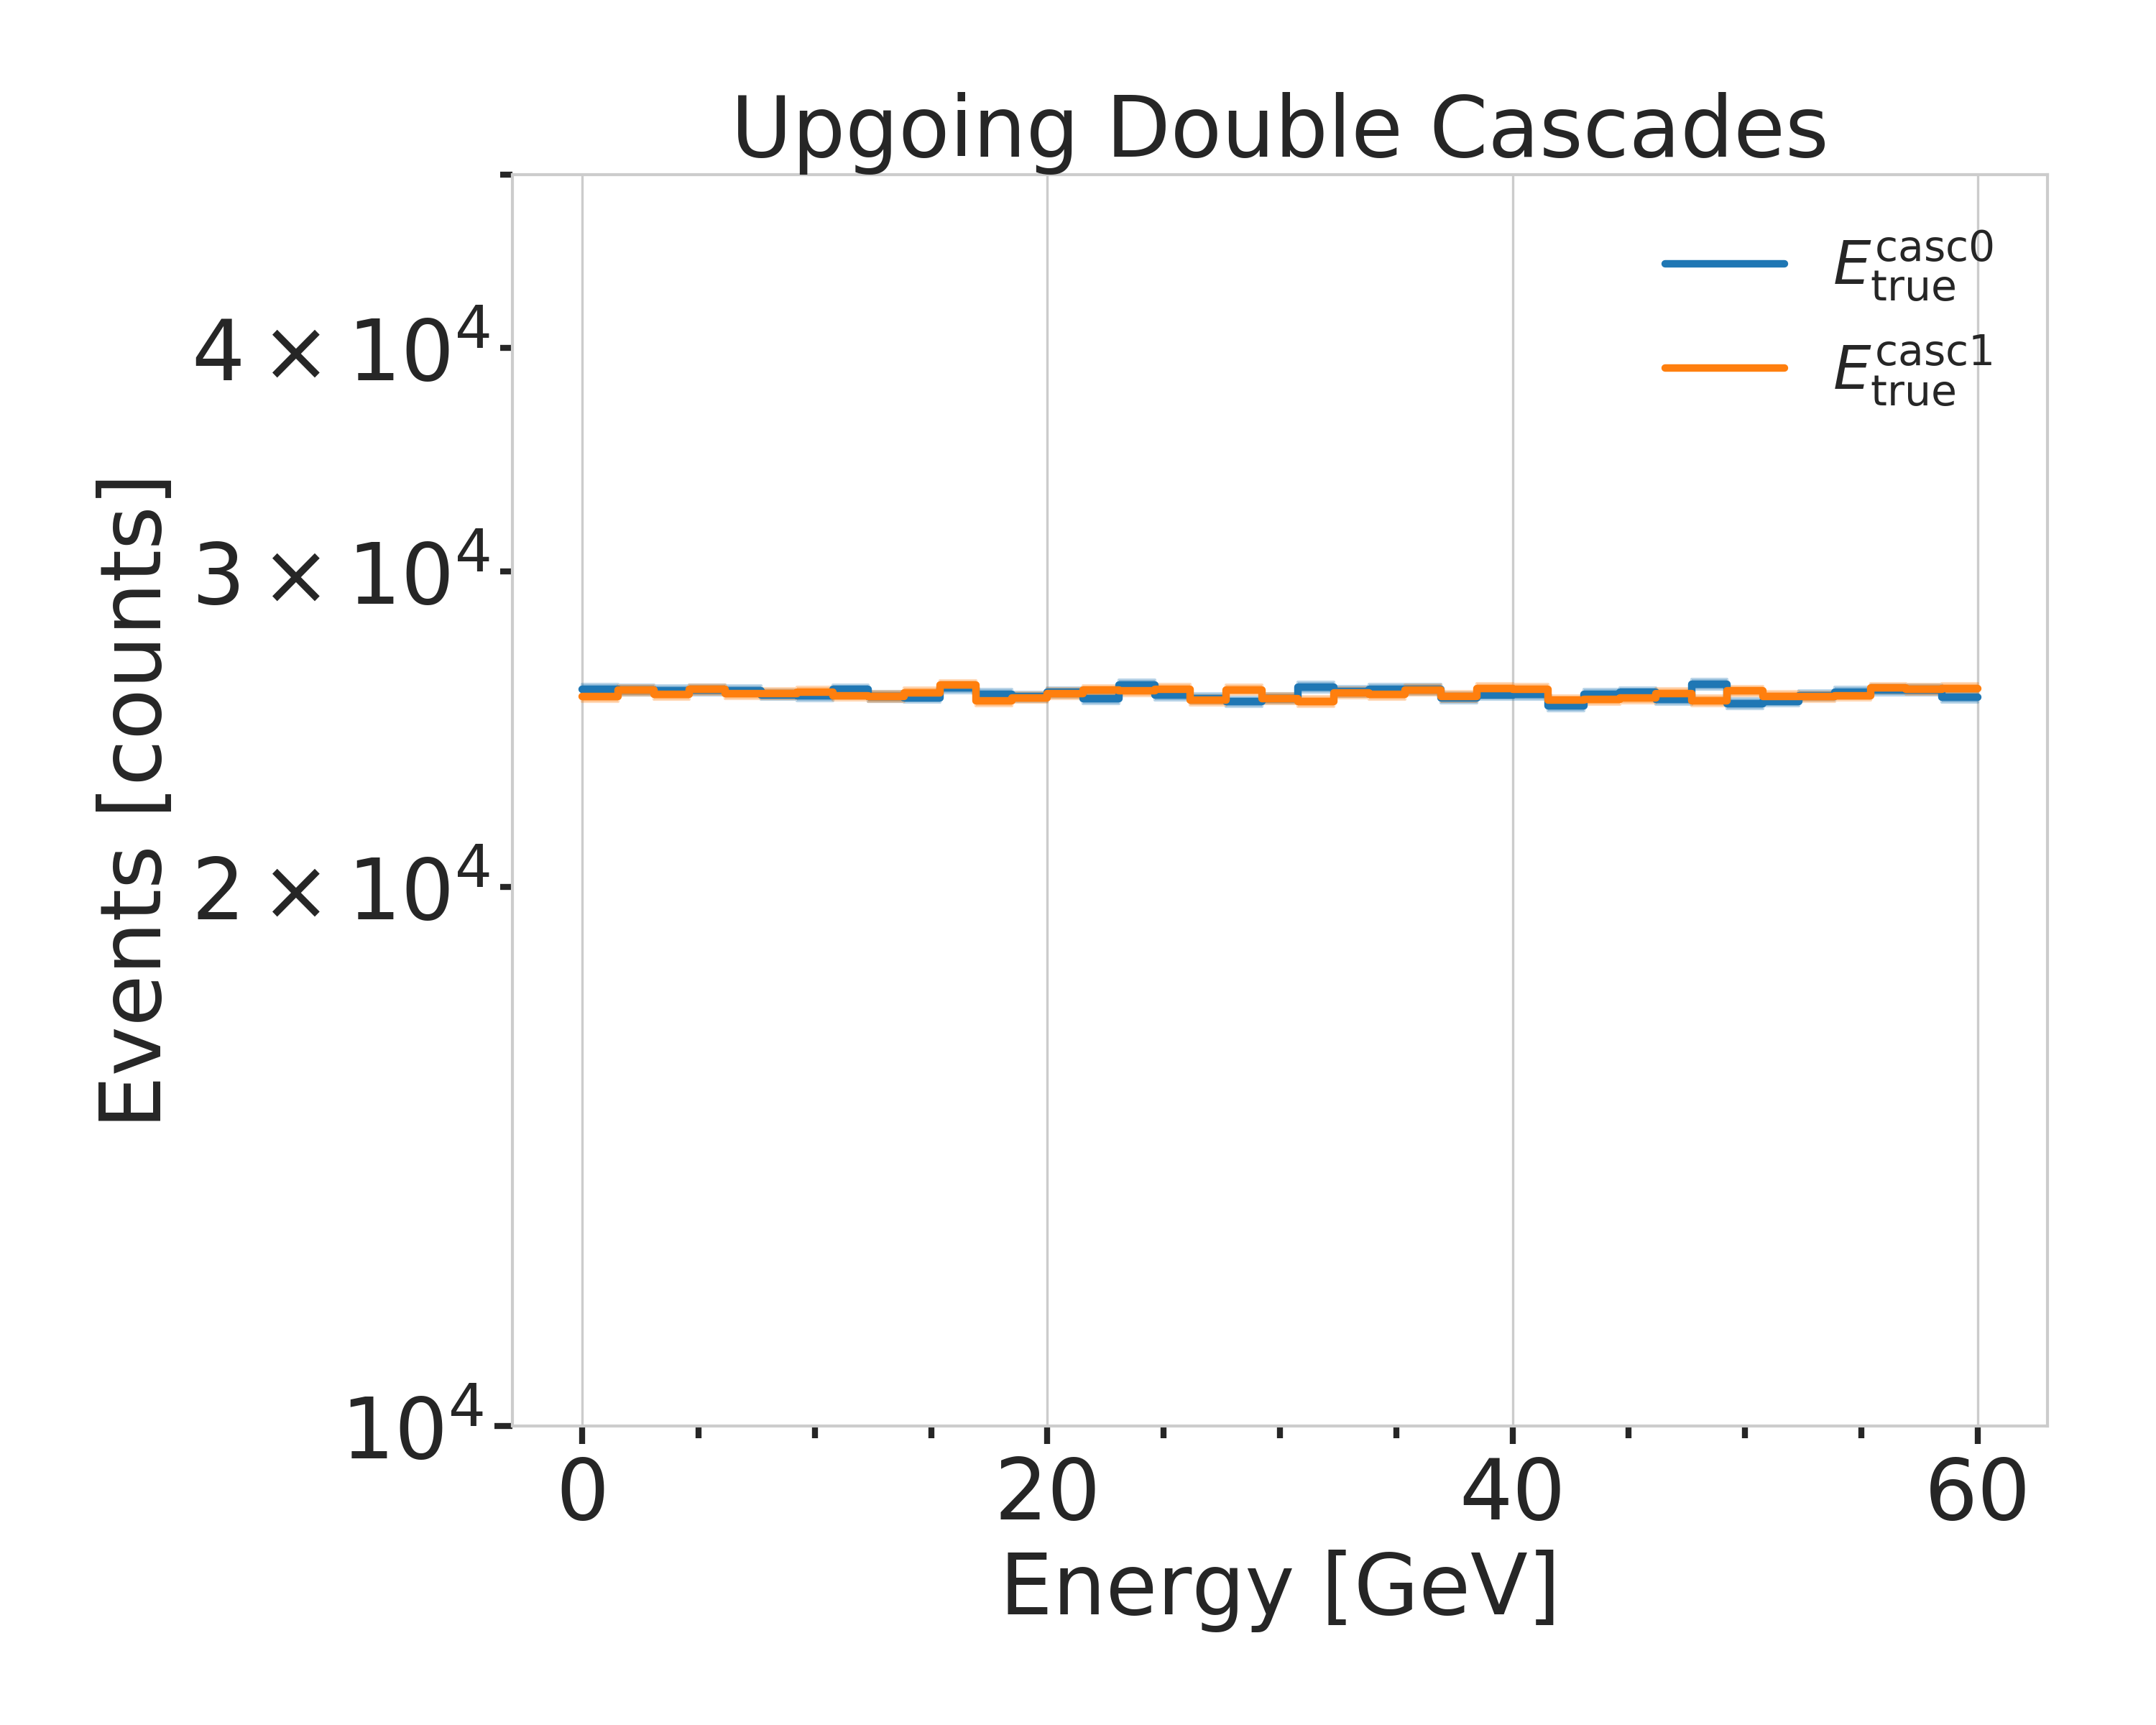
\includegraphics[width=.45\linewidth]{figures/upgoing_string_81_gen_level/1_d_distr_energies_clipped.png}
%     }
%     \subfloat[\labfig{horizontal_gen_distris_depths}]{
%         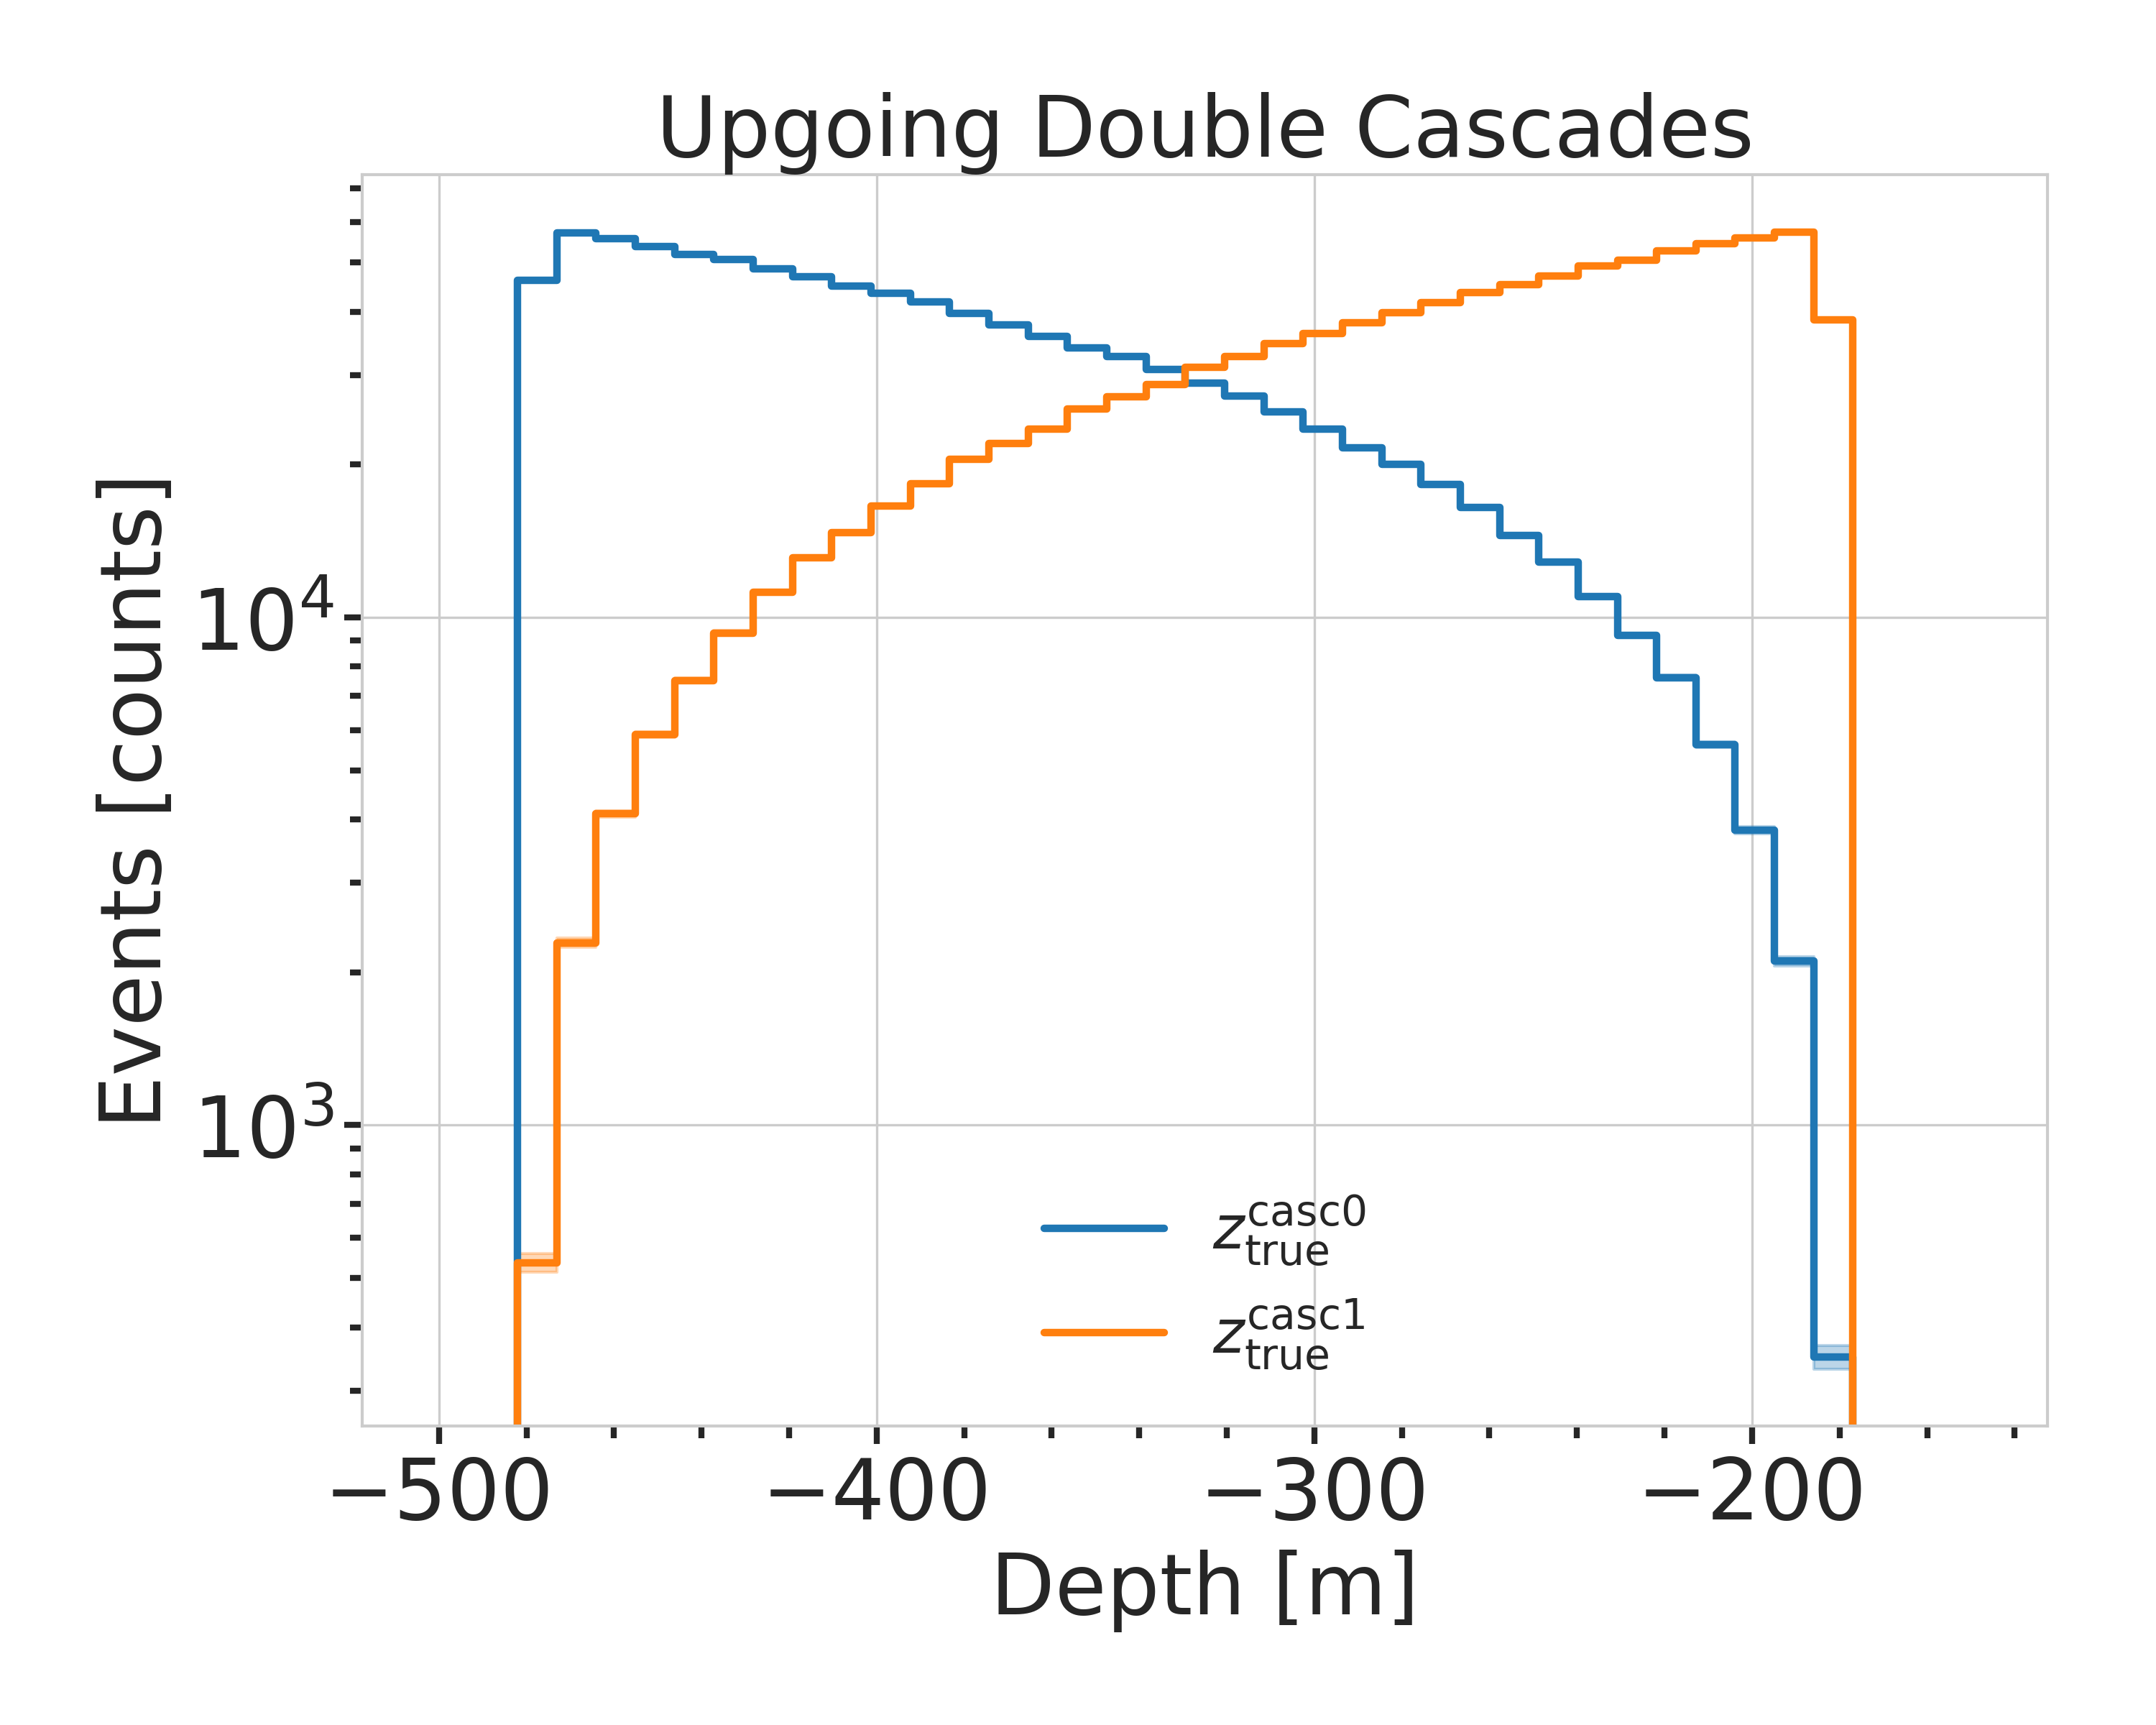
\includegraphics[width=.45\linewidth]{figures/upgoing_string_81_gen_level/1_d_distr_depths_clipped.png}
%     }
%     \\[-2.5ex]
%     \subfloat[\labfig{horizontal_gen_distris_decay_length}]{
%         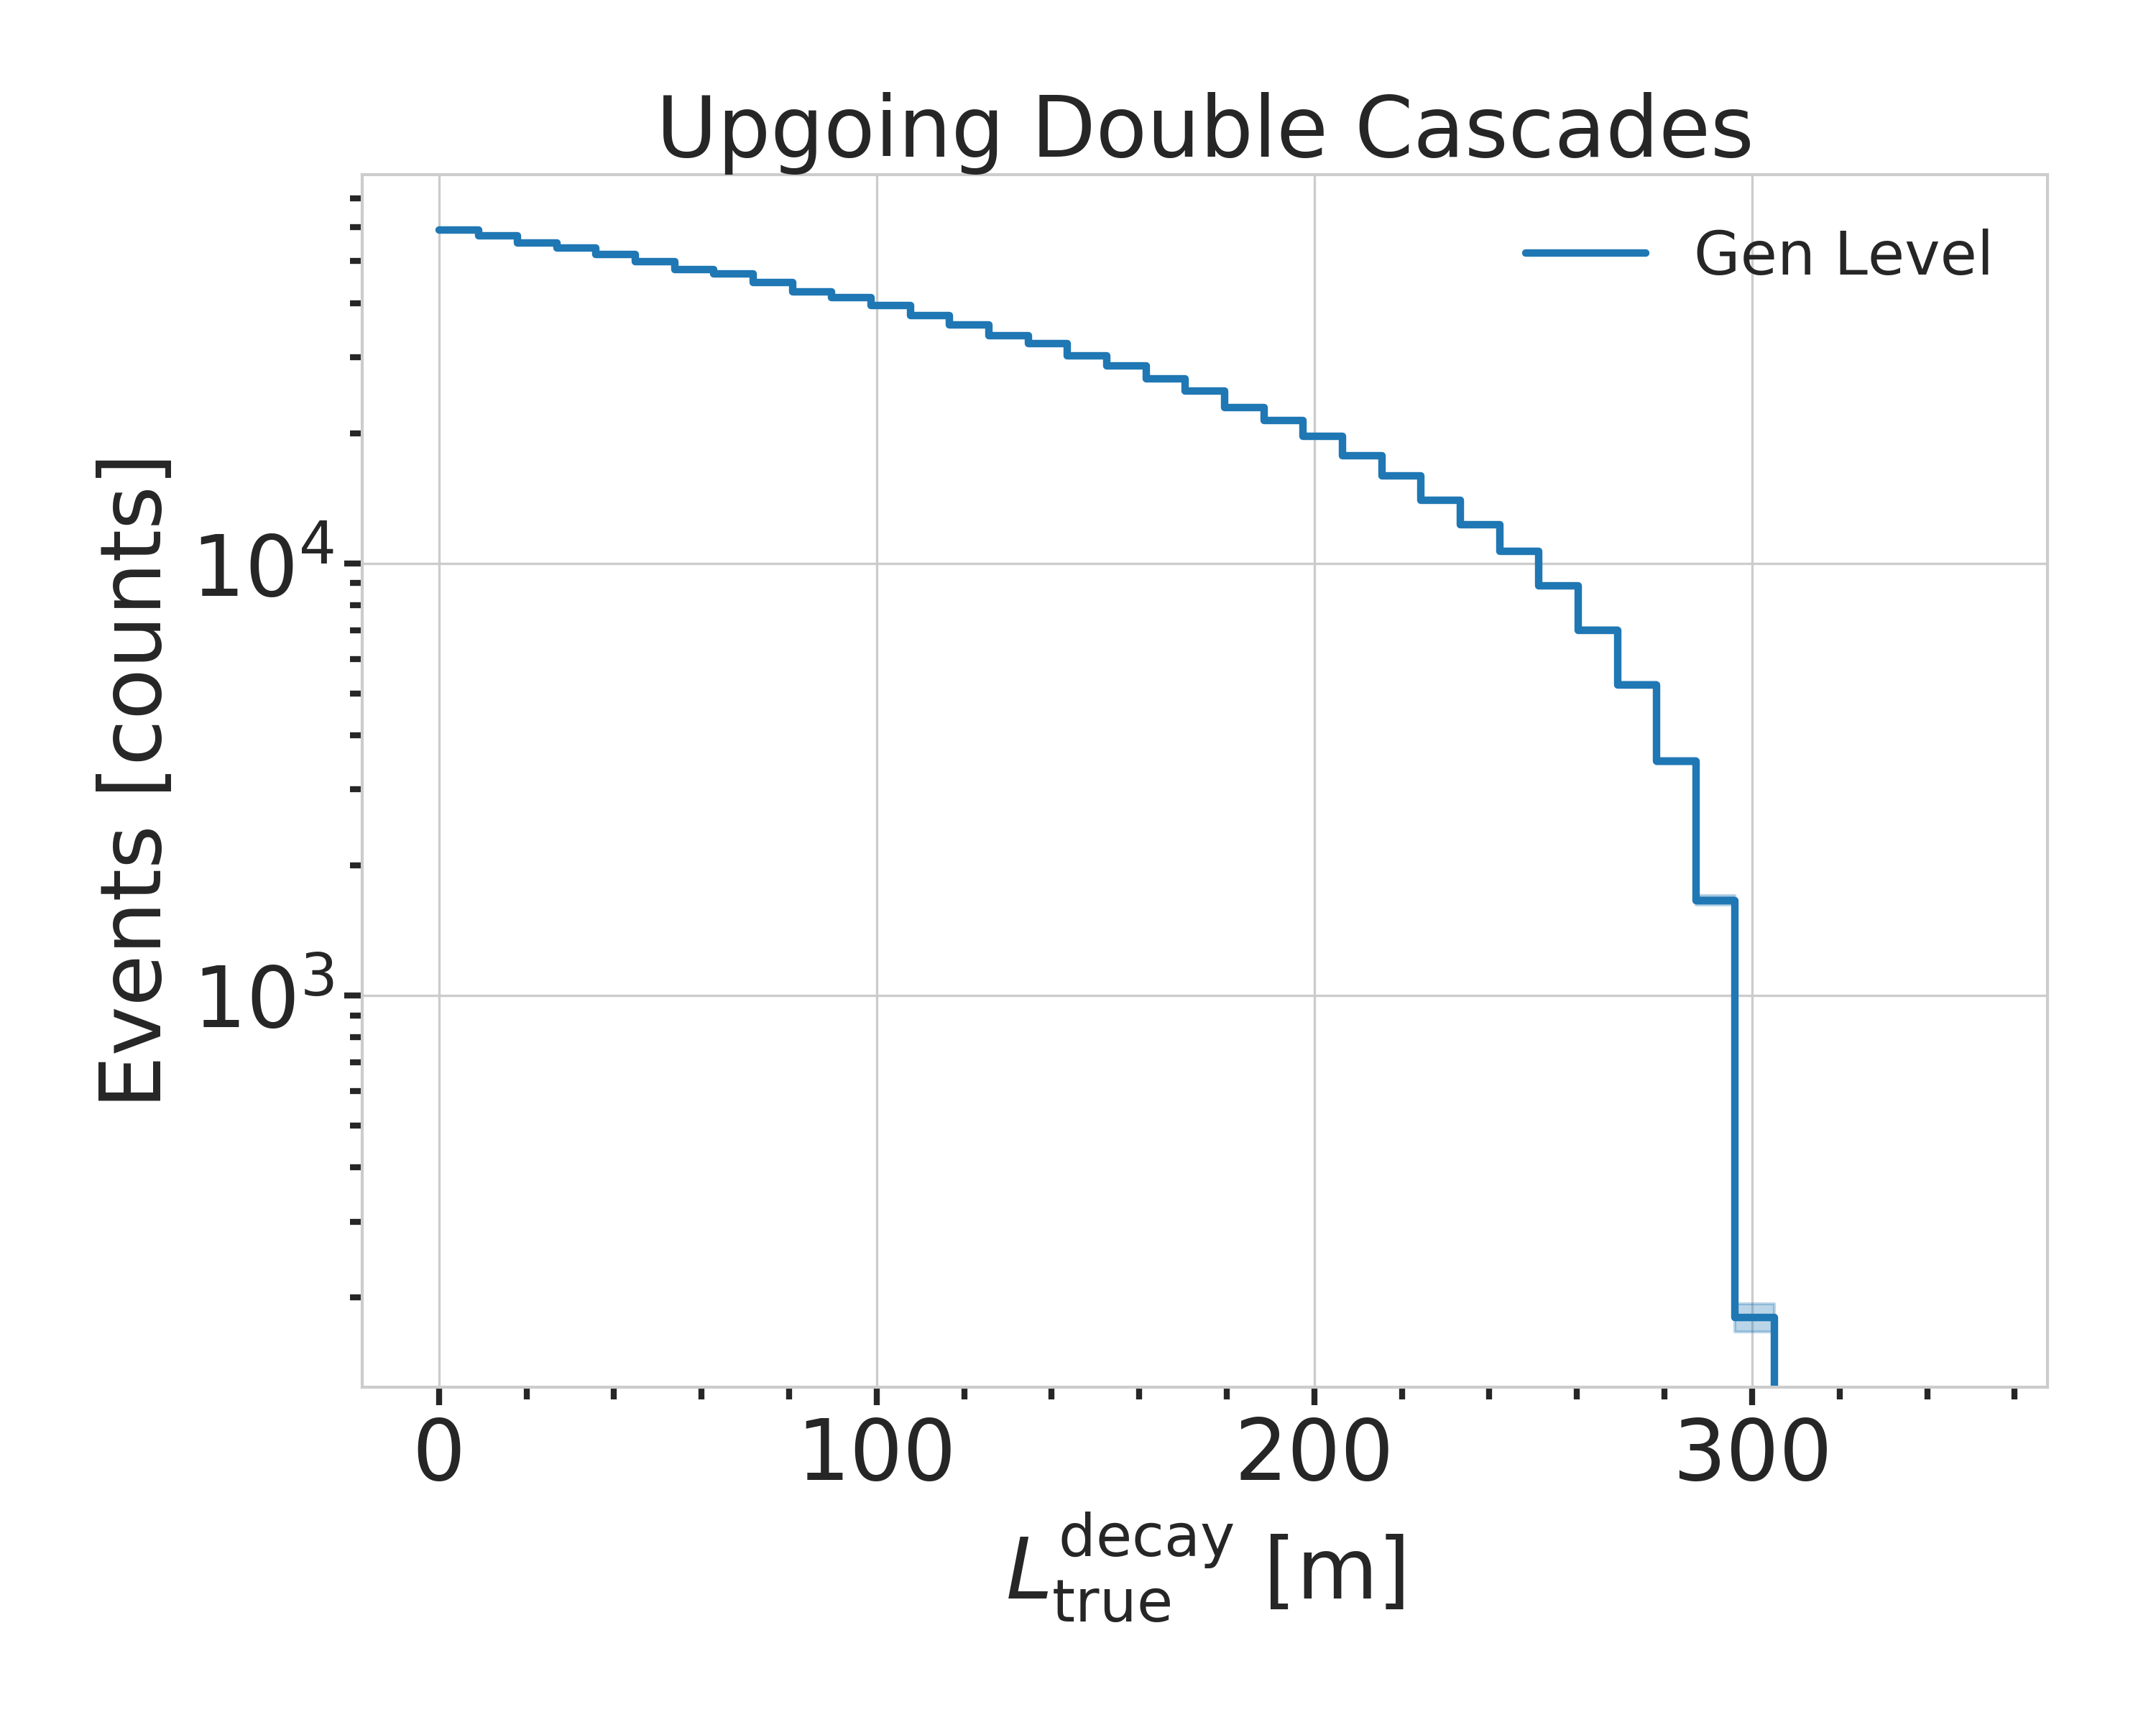
\includegraphics[width=.45\linewidth]{figures/upgoing_string_81_gen_level/1_d_distr_true_decay_length_clipped.png}
%     }
%     \subfloat[\labfig{horizontal_gen_distris_total_energy}]{
%         \includegraphics[width=.45\linewidth]{figures/upgoing_string_81_gen_level/1_d_distr_true_total_energy_clipped.png}
%     }
%     \caption{Generation level distributions of the 1k files, with 1k events each of set 194601. Only the parameters that are not fixed to a certain value are shown.}
%     \labfig{horizontal_gen_distris}
% \end{figure}

% \subsection{Final Level}



\section{Model Dependent Simulation} \labsec{model_specific_simulation}

\todo{Re-write/re-formulate this section (copied from HNL technote).}


\subsection{Custom LeptonInjector} \labsec{custom_leptoninjector}

Signal events are simulated using a \href{https://github.com/LeanderFischer/LeptonInjector-HNL/tree/main/LeptonInjector}{custom LeptonInjector (LI) tool} \sidecite{IceCube:2020tcq}, modified from its standard version to include the HNL particle and the description of the HNL decays needed to produce the double cascade signature (currently only $\nu_{\tau}$ related). In its SM work mode, LI injects a lepton and a cascade (under the general name \textit{Hadrons}) at the interaction vertex of the neutrino. Both objects have the same (x,y,z,t) coordinates. In the modified version, the lepton at the interaction vertex is replaced by the HNL. After a chosen distance the HNL is forced to decay. The decay is sampled from the kinematically accessible decay modes shown in \reffig{hnl_decay_modes_log_branching_ratio}.

A big addition to the standard LI is that the decay products of the HNL are added to the list of particles in the I3MCTree with a displaced position and delayed time from the interaction vertex. These daughter particles form a second cascade, not in the form of a \textit{Hadrons} object, but as the explicit particles forming the shower. The kinematics of the two-body decays are computed analytically, while the three-body decays are dealt with using MadGraph5. To do so, we randomly pick an event from a list that we generated for each three-body decay mode. Independent of the number of particles in the final state of the HNL decay, the kinematics are calculated/simulated at rest and then boosted along the HNL momentum. The decay mode is randomly chosen based on the mass dependent branching ratios shown in \reffig{hnl_decay_modes_log_branching_ratio}.

Each file is produced by running the \href{https://github.com/LeanderFischer/I3_HNL_Decay/blob/master/submission_scripts/process/process_Gen.py}{generation level processing script} using the filenumber as random seed and the above settings for the sampling distributions. The main part is calling the \textit{MultiLeptonInjector} module in \textit{volume mode} adding two generators (for $\nu_\tau$ and $\bar{\nu}_\tau$) with $50\%$ of the events. The generators are provided with the custom double-differential/total cross section splines described in \refsec{hnl_cross_sections} and the parameters defining the sampling distributions. For each frame \textit{OneWeight} and a reference weight are also calculated and stored using the \href{https://github.com/LeanderFischer/LeptonInjector-HNL/blob/main/LeptonInjector/python/hnl_weighting.py}{weighting functions} and a baseline atmospheric $\nu_\tau$ flux + oscillation spline. The weight will later be calculated inside of the analysis framework \href{https://github.com/icecube/pisa}{PISA}, based on the input OneWeight. In addition to the i3 file itself, a LeptonInjector configuration file is written which stores the needed information to produce event weights using LeptonWeighter. Optionally the script can also produce an hdf5 file with the same name in the same location. This will store a fixed set of keys, extracted from the i3 file.

We are using \textit{volume mode}, for the injection of the primary particle on a cylindrical volume. The main generation/sampling happens in \texttt{VolumeLeptonInjector::DAQ} inside \\ \texttt{LeptonInjector.cxx}. After writing the config (s) frame (currently not kept), the energy is sampled from a power law distribution, then the cosine(zenith) and azimuth angles are sampled from uniform distributions. The (x,y) position is sampled uniform in $r, \phi$ (for position on disk) and the z position is sampled from a uniform distribution. After the primary properties have been sampled the \textit{EventProperties} is created and handed over to the \texttt{FillTree} functions which is where the custom HNL simulation happens:

\subsubsection{Cross Sections} \labsec{hnl_cross_sections}


\todo{add varied total cross-section for a few background HNL events}

\begin{figure}
    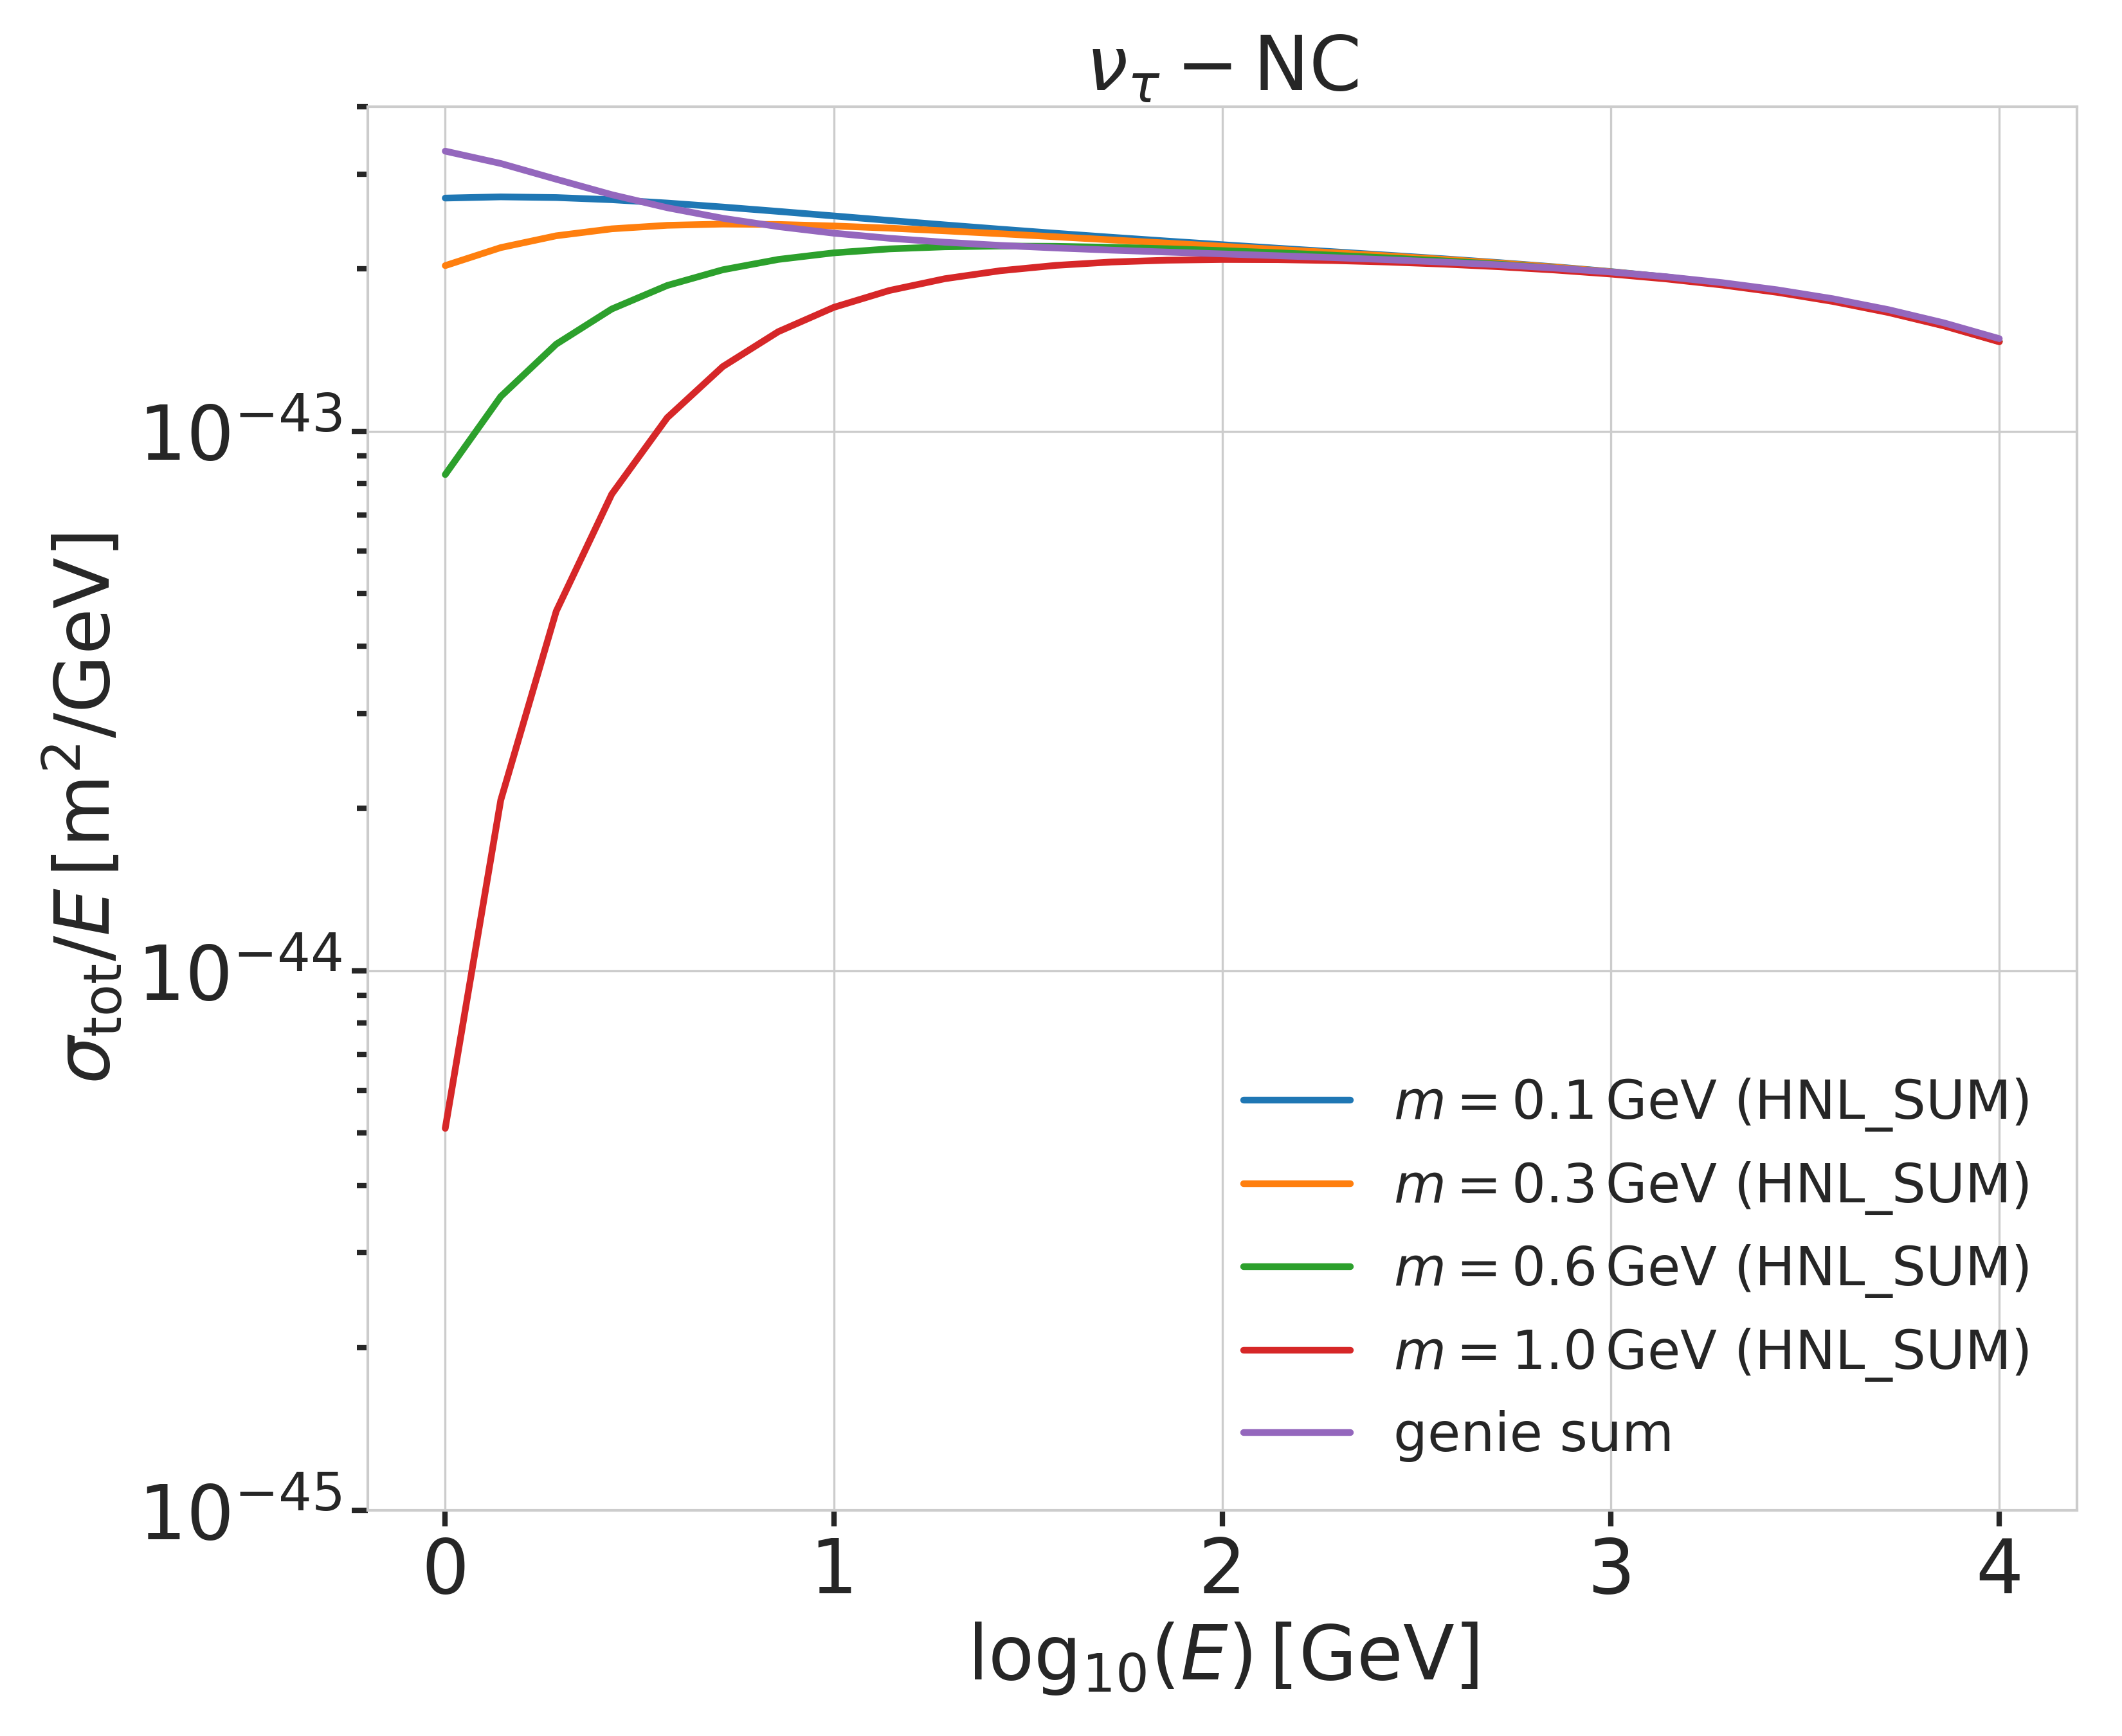
\includegraphics[width=.49\linewidth]{figures/hnl_simulation/cross_sections/custom_HNL_xsecs_final_SUM_flavorwise_total_xsecs_sigma-nutau-N-nc.png}
    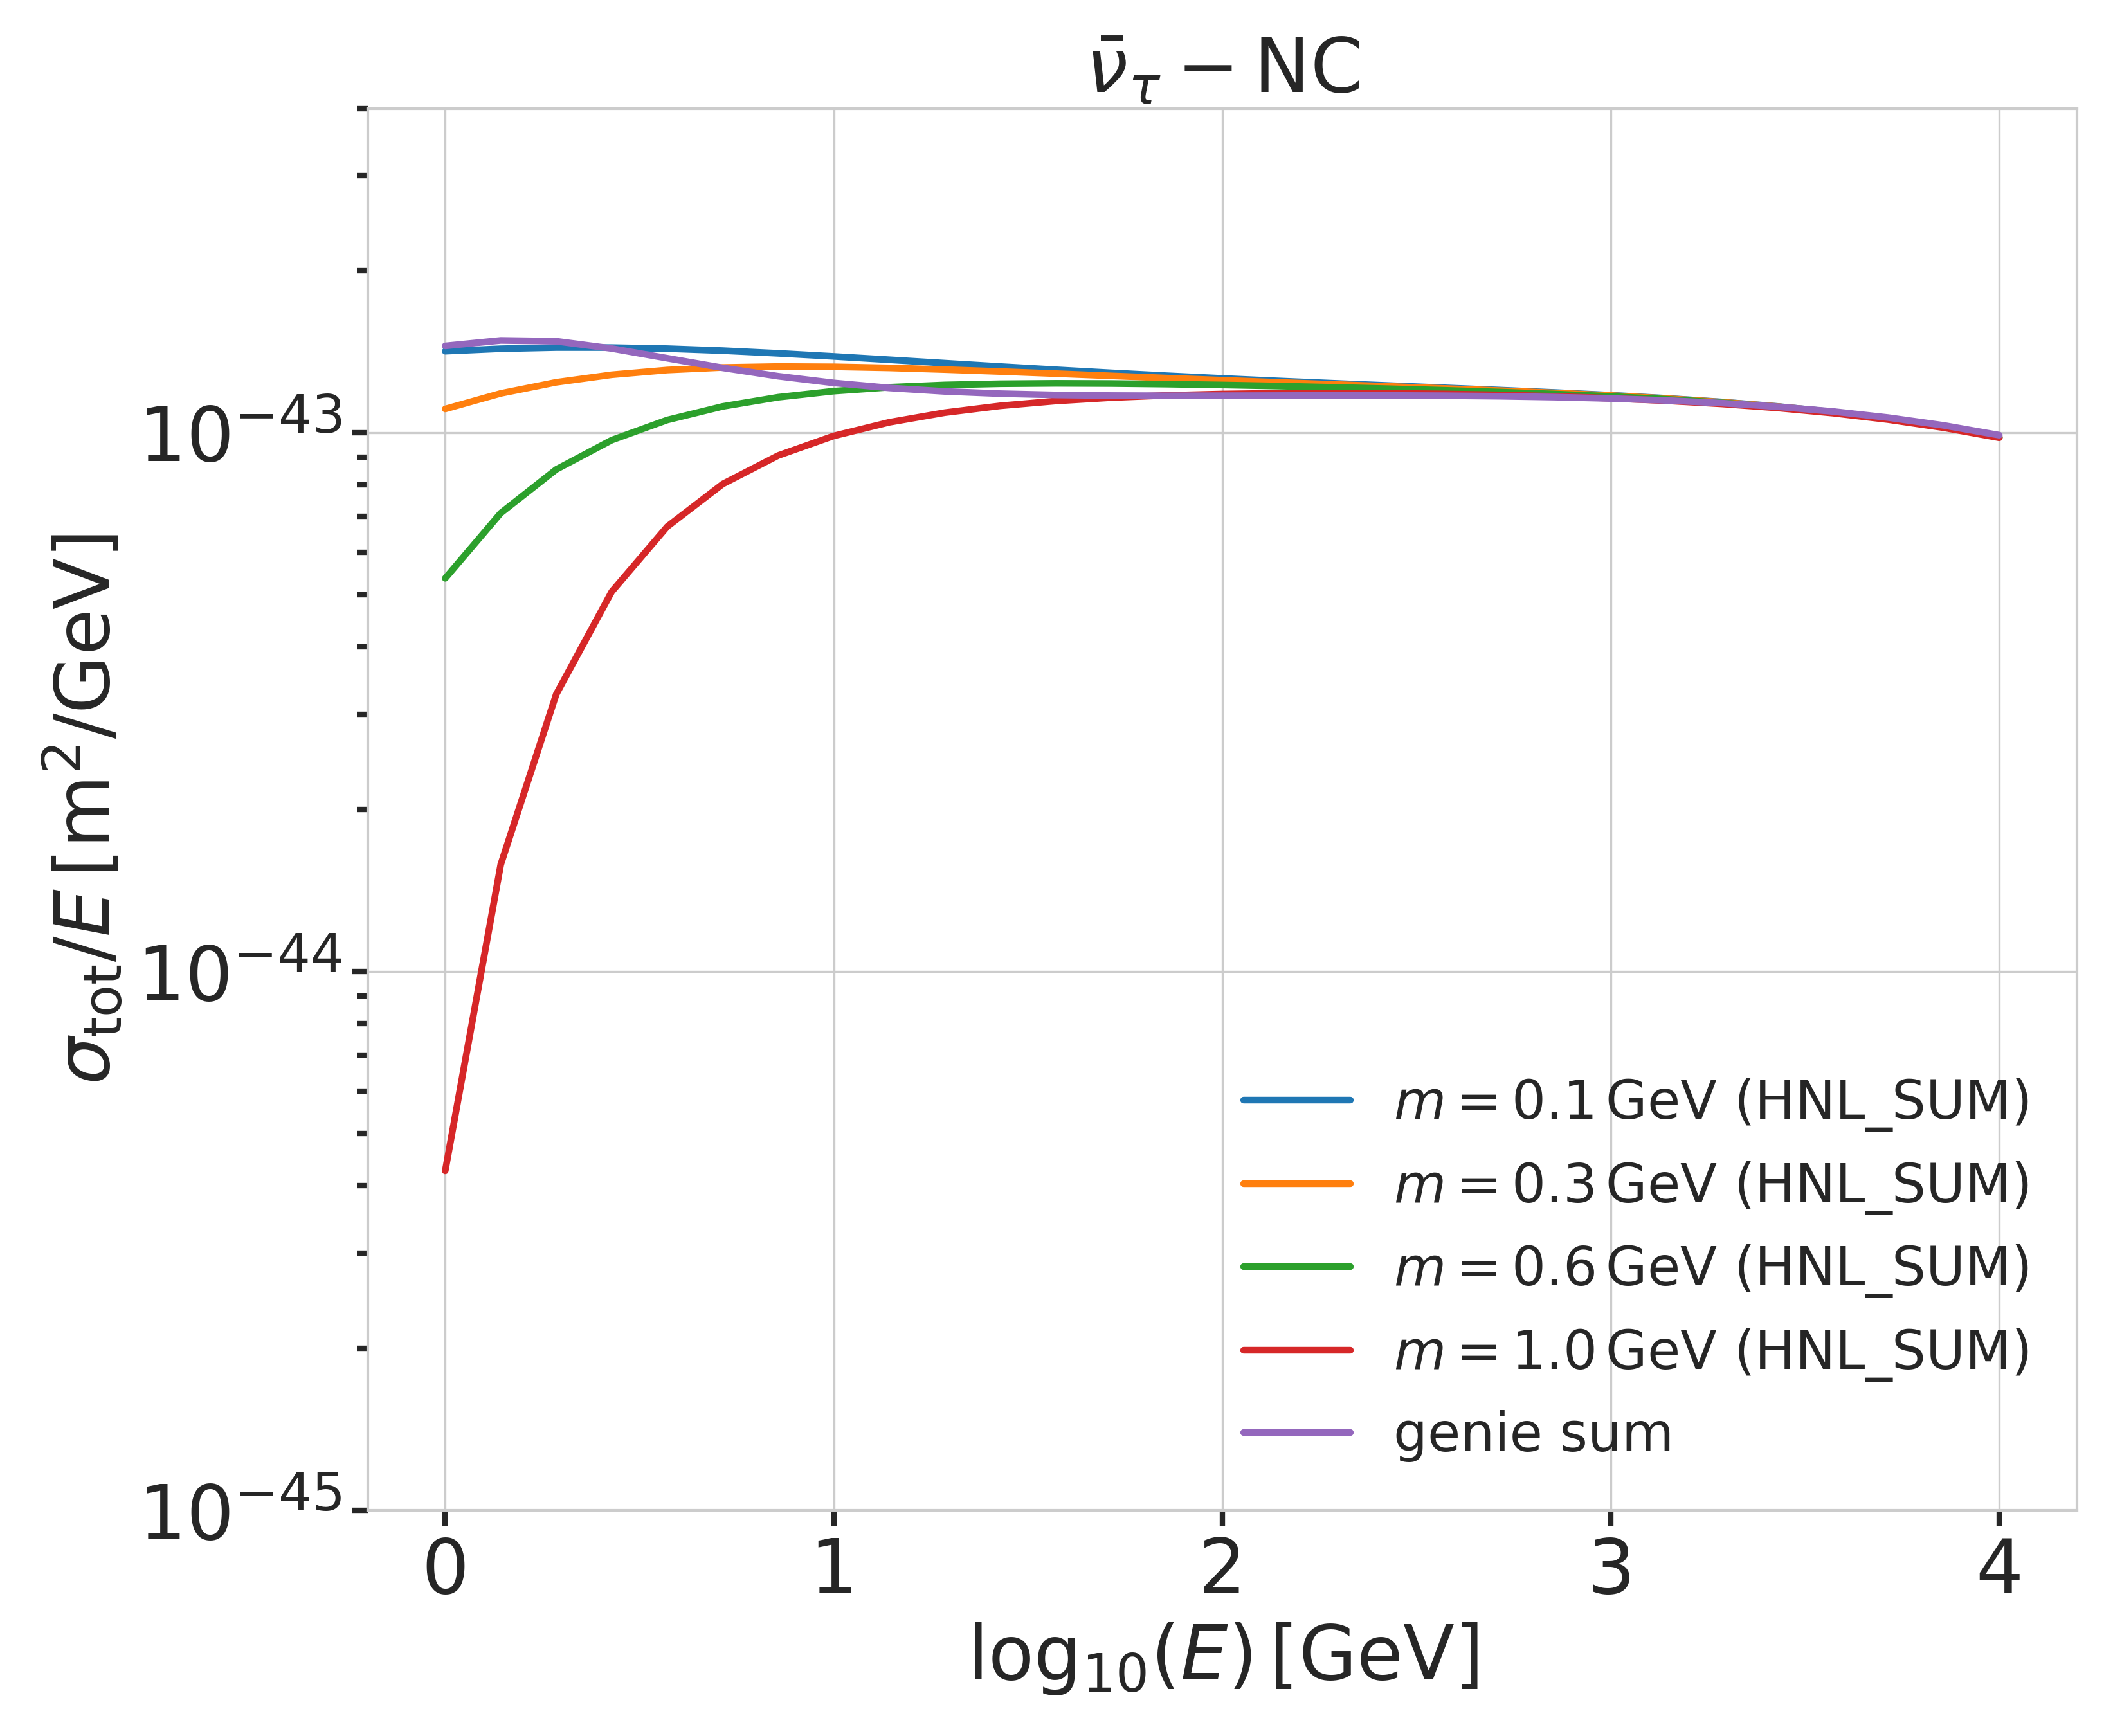
\includegraphics[width=.49\linewidth]{figures/hnl_simulation/cross_sections/custom_HNL_xsecs_final_SUM_flavorwise_total_xsecs_sigma-nutaubar-N-nc.png}
    \caption{Custom HNL total cross sections for the four target masses compared to the total ($\nu_\tau$/$\bar{\nu}_\tau$ neutral current) cross section used for SM neutrino simulation production with GENIE.}
    \labfig{custom_hnl_cross_sections}
\end{figure}

The cross sections are calculated using a \href{https://github.com/LeanderFischer/NuXSSplMkr/tree/massive_nu_nc_dis}{modified version} of Carlos Argüelles' \href{https://github.com/arguelles/NuXSSplMkr}{NuXSSplMkr}, which is a tool to calculate neutrino cross sections from parton distribution functions (PDFs) and then produce splines that can be read and used with IceCube software. The main modification to calculate the cross sections for the $\nu_\tau$ neutral current interaction into the new heavy mass state is the addition of a kinematic condition to ensure that there is sufficent energy to produce the heavy mass state. It is the same confition that needs to be fulfilled for the charged current case, where the outgoing lepton mass is non-zero. Following \sidecite{Levy:2004rk} (equation 7), the condition
\begin{equation}
    (1 + x \delta_N) h^2 - (x + \delta_{4}) h + x \delta_{4} \leq 0,
\end{equation}
is implemented for the neutral current case. Here $\delta_{4}=\frac{m_4^2}{s-M^2}$, $\delta_{N}=\frac{M^2}{s-M^2}$, and $h \overset{\textit{def}}{=} xy + \delta_{4}$, with $x, y$ being the Bjorken variables, $m_4$ and $M$ the mass of the heavy state and the target nucleon, respectively, and $s$ the center of mass energy squared. Since the (SM) neutrino background simulation used for this analysis was created using GENIE (version 2.12.8), interfaced through the IceCube software package \textit{genie-icetray}, with the \href{https://internal.dunescience.org/doxygen/classgenie_1_1GRV89LO.html}{GRV98LO} PDFs, those were added as \textit{GRV98lo\_patched} to the cross section spline maker, to ensure the best possibe agreement. Double-differential ($dsdxdy$) and total ($\sigma$) cross sections were produced for the four target HNL masses and then splined. The produced cross section splines are stored \href{https://github.com/LeanderFischer/LeptonInjector-HNL/tree/main/LeptonInjector/resources/cross_sections}{in the resources of the custom LeptonInjector module}. \reffig{custom_hnl_cross_sections} shows the total cross sections that were produced compared to the cross section used for the production of the SM $\nu_\tau/\bar{\nu}_\tau$ neutral current background simulation \todo{Add comparions of SM cross sections between NuXSSplMkr and genie}.


\subsubsection{Decay Channels}

\begin{figure}
    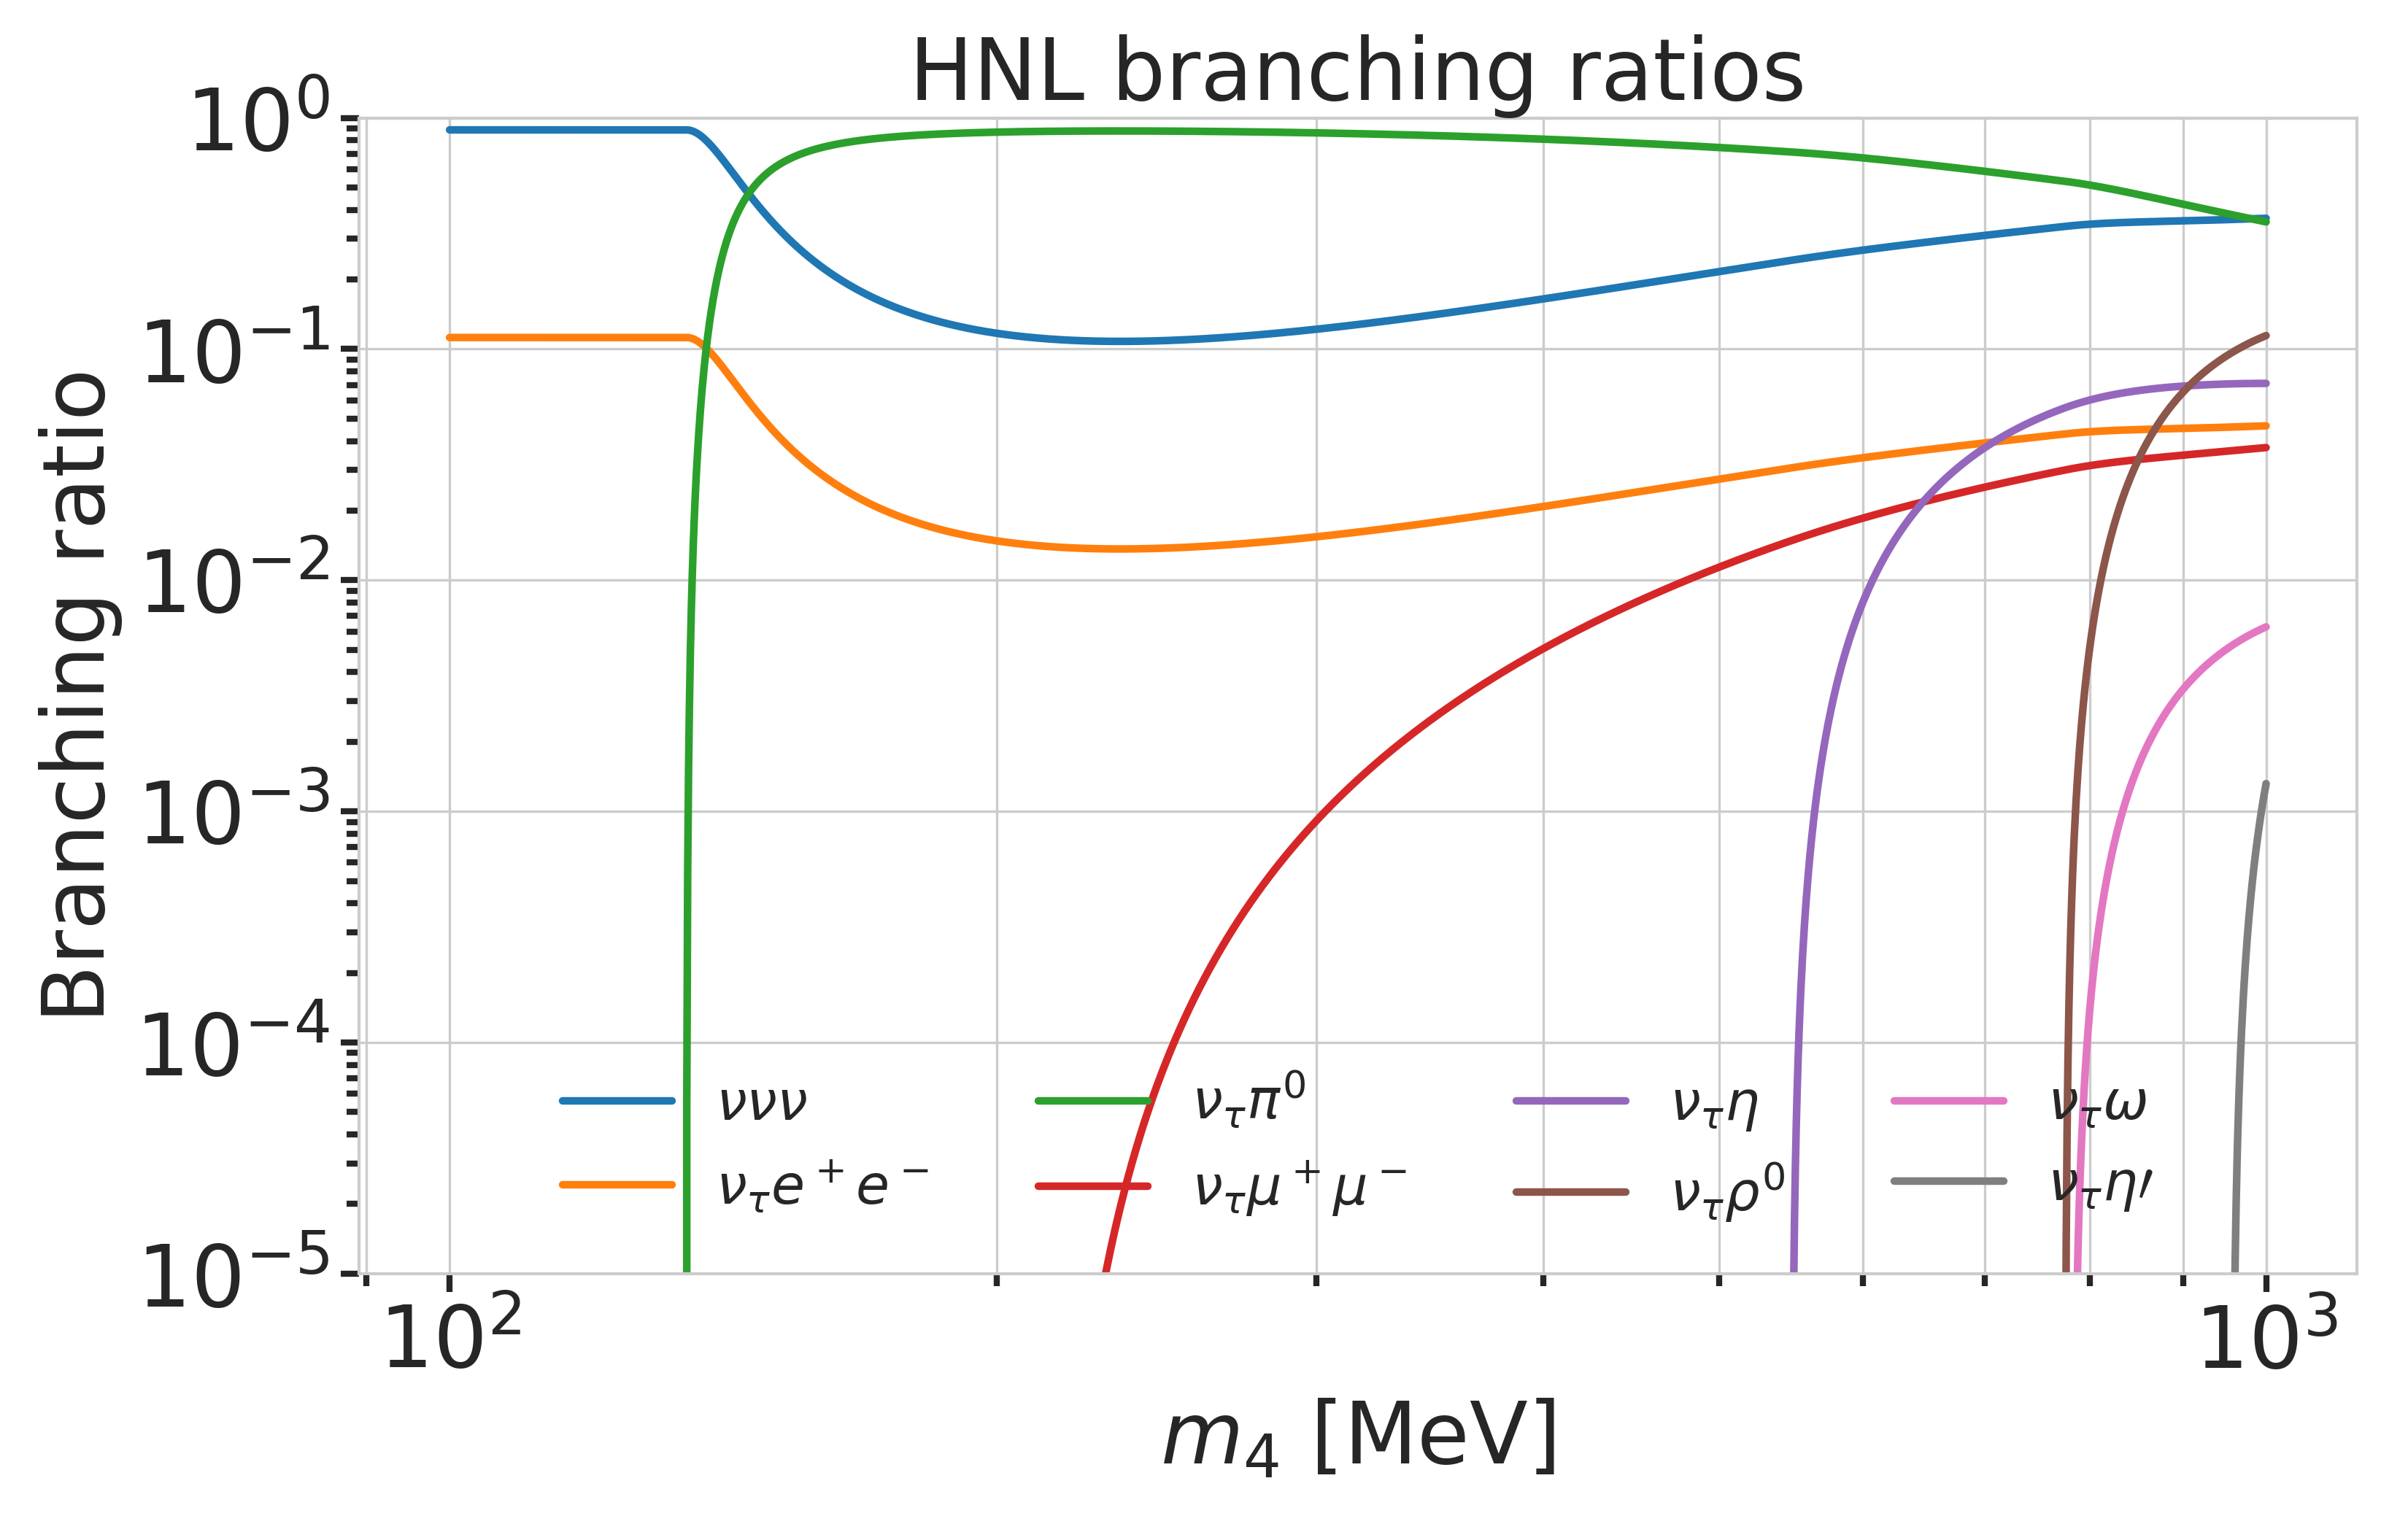
\includegraphics{hnl_simulation/decay_theory/branching_ratios_log_up_to_1.0_GeV.png}
    \caption{Branching ratios of the HNL within the mass range considered, calculated based on the results from \cite{Coloma:2020lgy}. Given the existing constraints on $|U_{e4}|^{2}$ and $|U_{\mu4}|^{2}$, we consider that the corresponding decay modes are negligible.}
    \labfig{hnl_decay_modes_log_branching_ratio}
\end{figure}

The accessible decay channels are dependent on the mass of the HNL and the allowed mixing. For this analysis, where only $|U_{\tau4}|^2 \neq 0$, the considered decay channels are listed in \reftab{hnl_decay_channels} and the corresponding branching ratios are shown in \reffig{hnl_decay_modes_log_branching_ratio}. The indiviudal branching ratio for a specific mass is calculated as $\mathrm{BR}_i(m_4)=\Gamma_i(m_4)/\Gamma_\mathrm{total}(m_4)$, where $\Gamma_\mathrm{total}(m_4)=\sum\Gamma_i(m_4)$. The formulas to calculate the decay width show up in multiple references, but we chose to match them to \sidecite{Coloma:2020lgy}, which also discusses the discrepencies in previous literature.

\begin{margintable}
    \footnotesize
    \begin{tabular} { lll }
        \hline\hline 
        \textbf{Channel} & \textbf{Opens} & \textbf{$\hat{\mathrm BR}$ [\%]} \\
        \hline\hline 
        $\nu_4 \rightarrow \nu_\tau \nu_\alpha \bar{\nu_\alpha}$ & \SI{0}{\MeV} & 100.0 \\
        $\nu_4 \rightarrow \nu_\tau e^+ e^-$ & \SI{1}{\MeV} & ? \\
        $\nu_4 \rightarrow \nu_\tau \pi^0$ & \SI{135}{\MeV} & ? \\
        $\nu_4 \rightarrow \nu_\tau \mu^+ \mu^-$ & \SI{211}{\MeV} & ? \\
        $\nu_4 \rightarrow \nu_\tau \eta$ & \SI{548}{\MeV} & ? \\
        $\nu_4 \rightarrow \nu_\tau \rho^0$ & \SI{770}{\MeV} & ? \\
        $\nu_4 \rightarrow \nu_\tau \omega$ & \SI{783}{\MeV} & ? \\
        $\nu_4 \rightarrow \nu_\tau \eta'$ & \SI{958}{\MeV} & ? \\
        \hline
    \end{tabular}
    \caption[xx]{xx}
    \labtab{hnl_decay_channels}
\end{margintable}



\paragraph{2-Body Decay Widths}

The decay to a neutral pseudoscalar mesons is
\begin{equation}
    \Gamma_{\nu_4 \rightarrow \nu_\tau P} = |U_{\tau4}|^2 \frac{G_F^2 m_4^3}{32\pi} f_P^2 (1-x_p^2)^2,
    \labeq{gamma_nu_P}
\end{equation}
with $x_P = m_P/m_4$ and
\begin{equation}
    f_{\pi^0} = \SI{0.130}{\GeV}, \hspace{1cm} f_{\eta} = \SI{0.0816}{\GeV}, \hspace{1cm} C_2 = f_{\eta'} = \SI{-0.0946}{\GeV},
    \labeq{gamma_nu_P_f_factors}
\end{equation}
while the decay to a neutral vector meson is given by
\begin{equation}
    \Gamma_{\nu_4 \rightarrow \nu_\tau V} = |U_{\tau4}|^2 \frac{G_F^2 m_4^3}{32\pi} \bigg(\frac{f_V}{m_V}\bigg)^2 g_V^2 (1+2x_V^2) (1-x_V^2)^2,
    \labeq{gamma_nu_V}
\end{equation}
with $x_V = m_V/m_4$,
\begin{equation}
    f_{\rho^0} = \SI{0.171}{\square\GeV}, \hspace{1cm} f_{\omega} = \SI{0.155}{\square\GeV},
    \labeq{gamma_nu_V_f_factors}
\end{equation}
and
\begin{equation}
    g_{\rho^0} = 1-2\sin^2{\theta_w}, \hspace{1cm} g_{\omega} = \frac{-2\sin^2{\theta_w}}{3}, \hspace{1cm} \sin^2{\theta_w} = 0.2229
    \labeq{gamma_nu_V_g_factors}
\end{equation}
\sidecite{codata2018}.


\paragraph{3-Body Decay Widths}

The (invisible) decay to three neutrinos is
\begin{equation}
    \Gamma_{\nu_4 \rightarrow \nu_\tau \nu_\alpha \bar{\nu_\alpha}} = |U_{\tau4}|^2 \frac{G_F^2 m_4^5}{192\pi^3},
    \labeq{gamma_nu_nu_nu}
\end{equation}
while the decay to two charged leptons (using $x_\alpha = (m_\alpha/m_4)^2)$ of the same flavor reads
\begin{equation}
    \Gamma_{\nu_4 \rightarrow \nu_\tau l_\alpha^+ l_\alpha^-} = |U_{\tau4}|^2 \frac{G_F^2 m_4^5}{192\pi^3} \big[ C_1 f_1(x_\alpha) + C_2 f_2(x_\alpha) \big],
    \labeq{gamma_nu_ll_full}
\end{equation}
with the constants defined as
\begin{equation}
    C_1 = \frac{1}{4}(1-4s_w^2+8s_w^4) , \hspace{1cm} C_2 = \frac{1}{2}(-s_w^2+2s_w^4),
    \labeq{gamma_nu_ll_c1_c2}
\end{equation} 
the functions as
\begin{equation}
    f_1(x_\alpha) = (1-14x_\alpha-2x_\alpha^2-12x_\alpha^3)\sqrt{1-4x_\alpha}+12x_\alpha^2(x_\alpha^2-1)L(x_\alpha),
    \labeq{gamma_nu_ll_f1}
\end{equation}
\begin{equation}
    f_2(x_\alpha) = 4[x_\alpha(2+10x_\alpha-12x_\alpha^2)\sqrt{1-4x_\alpha}+6x_\alpha^2(1-2x_\alpha+2x_\alpha^2)L(x_\alpha)],
    \labeq{gamma_nu_ll_f2}
\end{equation}
and
\begin{equation}
    L(x) = \ln \biggl( \frac{ 1-3x_\alpha-(1-x_\alpha)\sqrt{1-4x_\alpha} }{ x_\alpha(1+\sqrt{1-4x_\alpha}) } \biggr).
    \labeq{gamma_nu_ll_l}
\end{equation}


\subsection{MadGraph5 3-Body Decays} \labsec{madgraph_3body_decays}

The code to produce the 3-body decay kinematics is \href{https://launchpad.net/mg5amcnlo/3.0/3.3.x}{MadGraph4 v3.4.0} based on the decay diagrams calculated with \href{http://feynrules.irmp.ucl.ac.be/#FeynRules2.0}{FeynRules 2.0} using the Lagrangians derived in \sidecite{Coloma:2020lgy}. The Universal FeynRules Outpur (UFO) from \texttt{effective\_HeavyN\_Majorana\_v103} were used for our calculation. For each meass and corresponding decay channel, we produce $1e06$ decay kinematic variations (rest frame) and store those in a text file. 


\subsection{Sampling Distributions}

This is the description of the signal simulation generator used to (re-)start simulation production in December 2023. The underlying sampling distributions are listed in \reftab{HNL_sampling_distributions}. Judging from how the generation/processing efficiency was for the 190607 set, we target $1e04$ files per set with $5e05$ events per file at generation, resulting in a maximum of $5e09$ events per set at generation level. Note here that the actual number of events per set at generation might be a little lower since some events won't be allowed if they don't have enough energy to produce the HNL.

\begin{table}
    \centering
    \begin{tabular} { lll }
        \hline \hline 
        \textbf{Variable} & \textbf{Distribution} & \textbf{Range/Value} \\
        \hline \hline 
        energy & $E^{-2}$ & [\SI{2}{\GeV}, \SI{1e4}{\GeV}] \\
        zenith & uniform (in $\cos(\theta)$) & [\SI{180}{\degree}, \SI{80}{\degree}] \\
        azimuth & uniform & [\SI{0}{\degree}, \SI{360}{\degree}] \\
        vertex $x,y$ & uniform & $r$=\SI{600}{\metre} \\
        vertex $z$ & uniform & [-600, 0]\si{\metre} \\
        $m_\mathrm{4}$ & fixed & [0.3, 0.6, 1.0]\si{\GeV} \\
        $L_\mathrm{decay}$ & $L^{-1}$ & [0.0004, 1000]\si{\metre} / [1, 1000]\si{\metre} \\
        \hline
    \end{tabular}
    \caption[xx]{Sampling distributions of HNL simulation generation.}   
    \labtab{hnl_realistic_set_sampling_distributions}
\end{table}


\subsection{Weighting Scheme}

The weighting for the HNL signal simulation happens in a \href{https://github.com/icecube/pisa/blob/master/pisa/stages/aeff/weight_hnl.py}{custom stage of PISA}. The only input is the stored OneWeight and the variable physics parameter $|U_{\tau4}|^2$, which is the mixing strength of the new heavy mass state and the tau sector. The custom re-weighting is needed to go from the used sampling PDF (1/L with fixed range in lab frame decay length) to the target PDF (exponential defined by proper lifetime of the HNL). For each event the re-weighting factor is calculated using the gamma factor
\begin{equation}
    \gamma = \frac{\sqrt{E_\mathrm{kin}^2+m_\mathrm{HNL}^2}}{m_\mathrm{HNL}},
    \labeq{gamma_factor}
\end{equation}
with the HNL mass $m_\mathrm{HNL}$ and it's kinetic energy $E_\mathrm{kin}$. The speed of the HNL is calculated as
\begin{equation}
    v = c \cdot \sqrt{1 - \frac{1}{\gamma^2}},
    \labeq{lorentz_speed}
\end{equation}
where $c$ is the speed of light. With these the lab frame decay length range can be converted into the rest frame lifetime range for each event
\begin{equation}
    \tau_\mathrm{min/max} = \frac{s_\mathrm{min/max}}{v\cdot\gamma}.
\end{equation}
The proper lifetime of each HNL event can be calculated using the total decay width $\Gamma_\mathrm{total}$ shown in \reffig{hnl_decay_modes_log_decay_width} and the chosen mixing strength $|U_{\tau4}|^2$ as
\begin{equation}
    \tau_\mathrm{proper} = \frac{\hbar}{\Gamma_\mathrm{total}(m_\mathrm{HNL}) \cdot |U_{\tau4}|^2},
    \labeq{proper_lifetime}
\end{equation}
where $\hbar$ is the reduced Planck constant. Since the decay length/lifetime of the events is sampled from an inverse distribution instead of an exponential as it would be expected from a particle decay we have to re-weight accordingly to achieve the correct decay length/lifetime distribution. This is done by using the wanted exponential distribution
\begin{equation}
    \mathrm{PDF}_\mathrm{exp} = \frac{1}{\tau_\mathrm{proper}} \cdot e^{\frac{-\tau}{\tau_\mathrm{proper}}},
    \labeq{pdf_exponential}
\end{equation}
and the inverse distribution that was sampled from
\begin{equation}
    \mathrm{PDF}_\mathrm{inv} = \frac{1}{\tau \cdot (\ln(\tau_\mathrm{max}) - \ln(\tau_\mathrm{min}))}.
    \labeq{pdf_inverse}
\end{equation}
The lifetime re-weighting factor is calculated as
\begin{equation}
    w_\mathrm{lifetime} = \frac{\mathrm{PDF}_\mathrm{exp}}{\mathrm{PDF}_\mathrm{inv}} = \frac{\Gamma_\mathrm{total}(m_\mathrm{HNL}) \cdot |U_{\tau4}|^2}{\hbar} \cdot \tau \cdot (\ln(\tau_\mathrm{max}) - \ln(\tau_\mathrm{min})) \cdot e^{\frac{-\tau}{\tau_\mathrm{proper}}}.
    \labeq{weight_lifetime}
\end{equation}
Adding another factor of $|U_{\tau4}|^2$ to account for the mixing at the interaction vertex the total re-weighting factor becomes
\begin{equation}
    w_\mathrm{total} = |U_{\tau4}|^2 \cdot w_\mathrm{lifetime},
    \labeq{weight_full}
\end{equation}
which can be applied on top of flux and oscillation weight to get the final HNL weight for a given mixing (and mass).

\subsection{Generation Level Distributions}
